% Section content template for individual Educative lessons
% This file contains the actual content for a specific section
% Generated from Educative API section content

% Section: Unique IDs with Causality
% Section ID: 5836711686307840
% Section Slug: unique-ids-with-causality
% Generated: 2025-12-07T17:30:59.303215

\subsection{Causality}\label{5lR72LzoGMpj6XzZ2e0BH}
\\
In the \href{https://www.educative.io/courses/grokking-the-system-design-interview/design-of-a-unique-id-generator}{previous} lesson, we generated unique IDs to differentiate between various events. Apart from having unique identifiers for events, we're also interested in finding the sequence of these events. Let 's consider an example where Peter and John are two Twitter users. John posts a comment (event A), and Peter replies to John's comment (event B). Event
B is dependent on event A and can't happen before it. The events are not concurrent here.
\\
We can also have concurrent events---that is, two events that occur independently of each other. For example, if Peter and John comment on two different Tweets, there's no happened-before relationship or causality between them. It 's essential to identify the dependence of one event over the other but not in the case of concurrent events.
\begin{quote}
\textbf{Note:} The scenario described above can also be handled by assigning a unique ID and encoding the dependence of events using a social graph. We might also use a separate time data structure and a simple unique ID. However, we want a unique ID to do double duty---provide unique identification and also help with the causality of events.
\end{quote}
\\
The following slides provide a visualization of concurrent and nonconcurrent events.

\begin{figure}[htbp]
 \centering
 \begin{subfigure}[b]{0.48\textwidth}
 \centering
 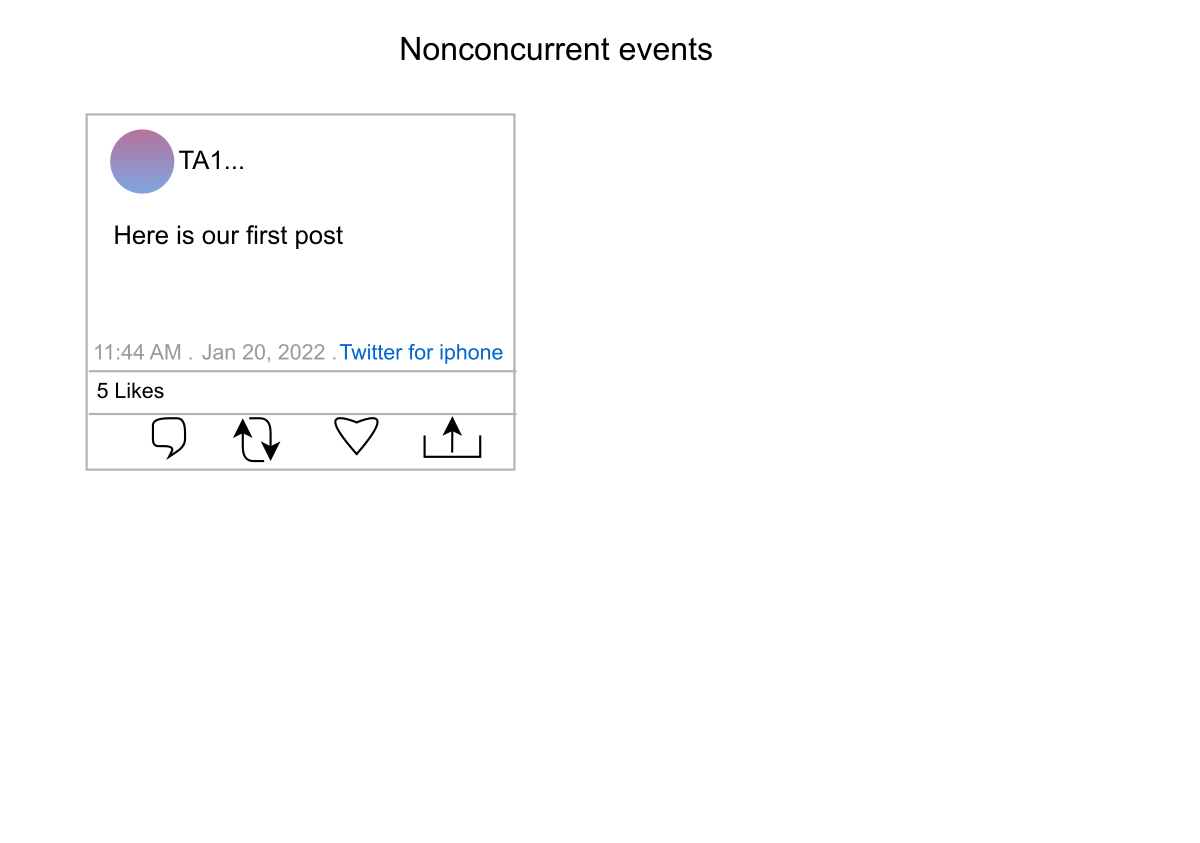
\includegraphics[width=\textwidth]{Images/chapter_12/section_5836711686307840/6284923883487232.png}
 \end{subfigure}
 \hfill
 \begin{subfigure}[b]{0.48\textwidth}
 \centering
 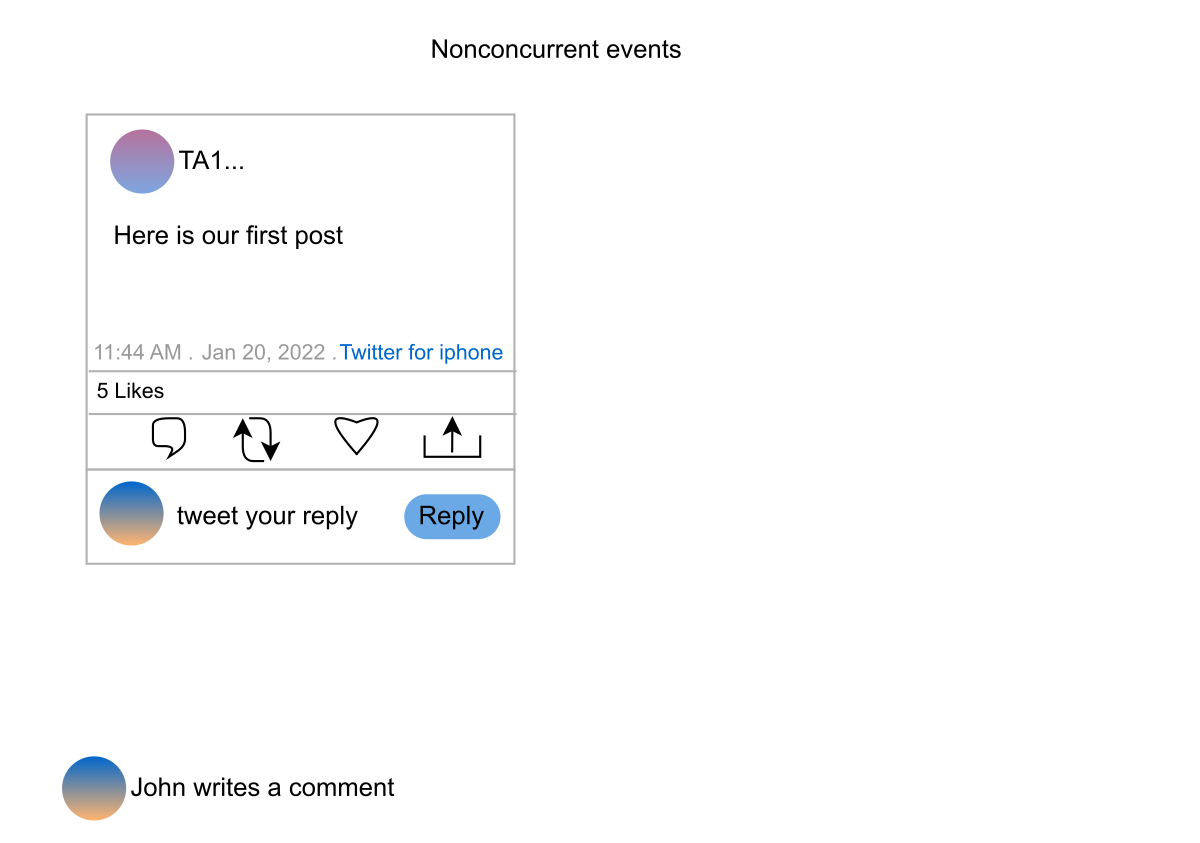
\includegraphics[width=\textwidth]{Images/chapter_12/section_5836711686307840/6507345811341312.png}
 \end{subfigure}
\end{figure}

\begin{figure}[htbp]
 \centering
 \begin{subfigure}[b]{0.48\textwidth}
 \centering
 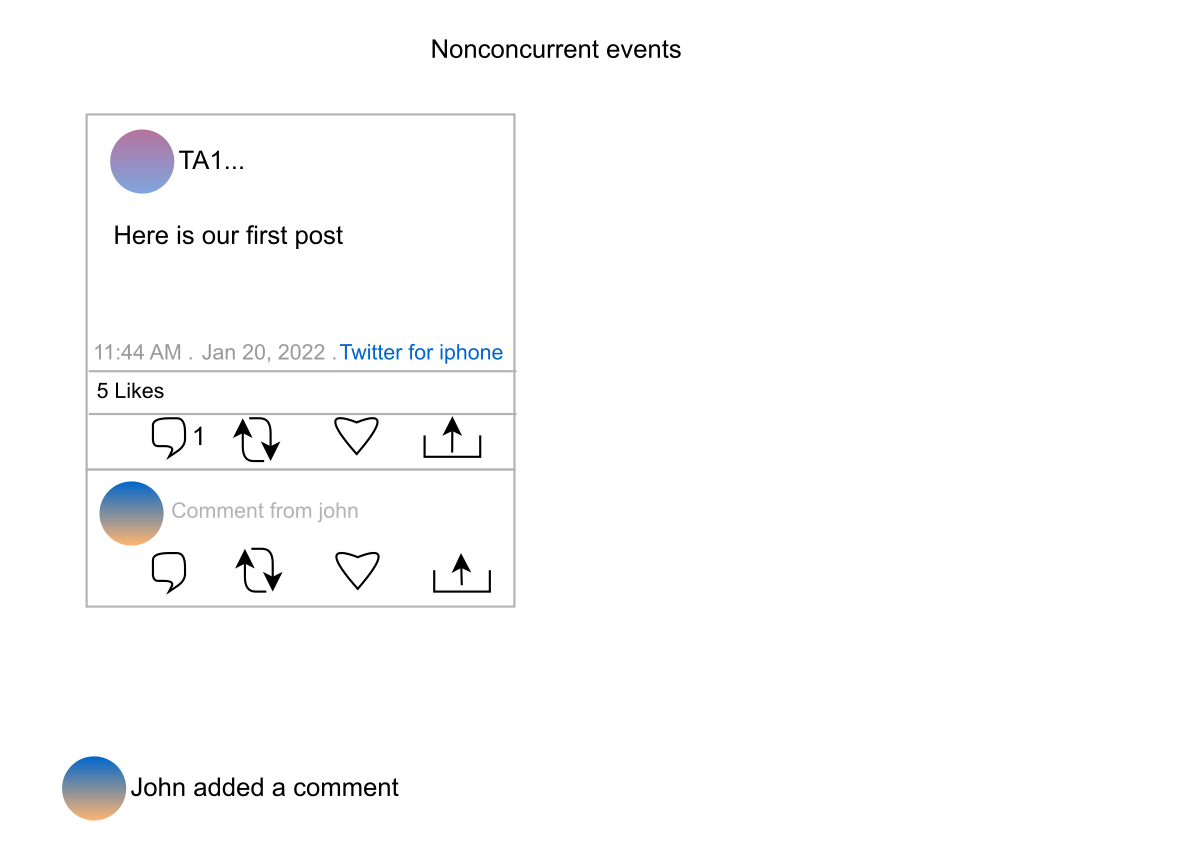
\includegraphics[width=\textwidth]{Images/chapter_12/section_5836711686307840/6428893737385984.png}
 \end{subfigure}
 \hfill
 \begin{subfigure}[b]{0.48\textwidth}
 \centering
 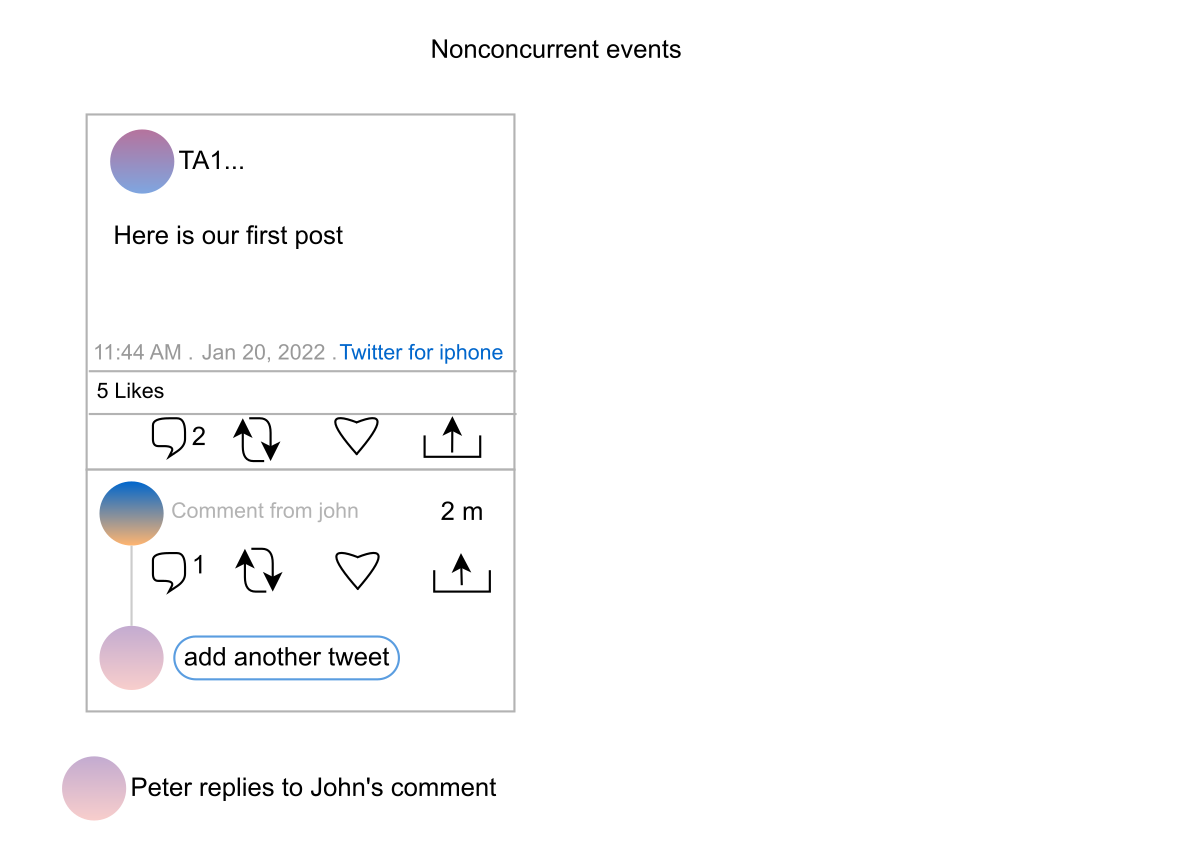
\includegraphics[width=\textwidth]{Images/chapter_12/section_5836711686307840/4852341300002816.png}
 \end{subfigure}
\end{figure}

\begin{figure}[htbp]
 \centering
 \begin{subfigure}[b]{0.48\textwidth}
 \centering
 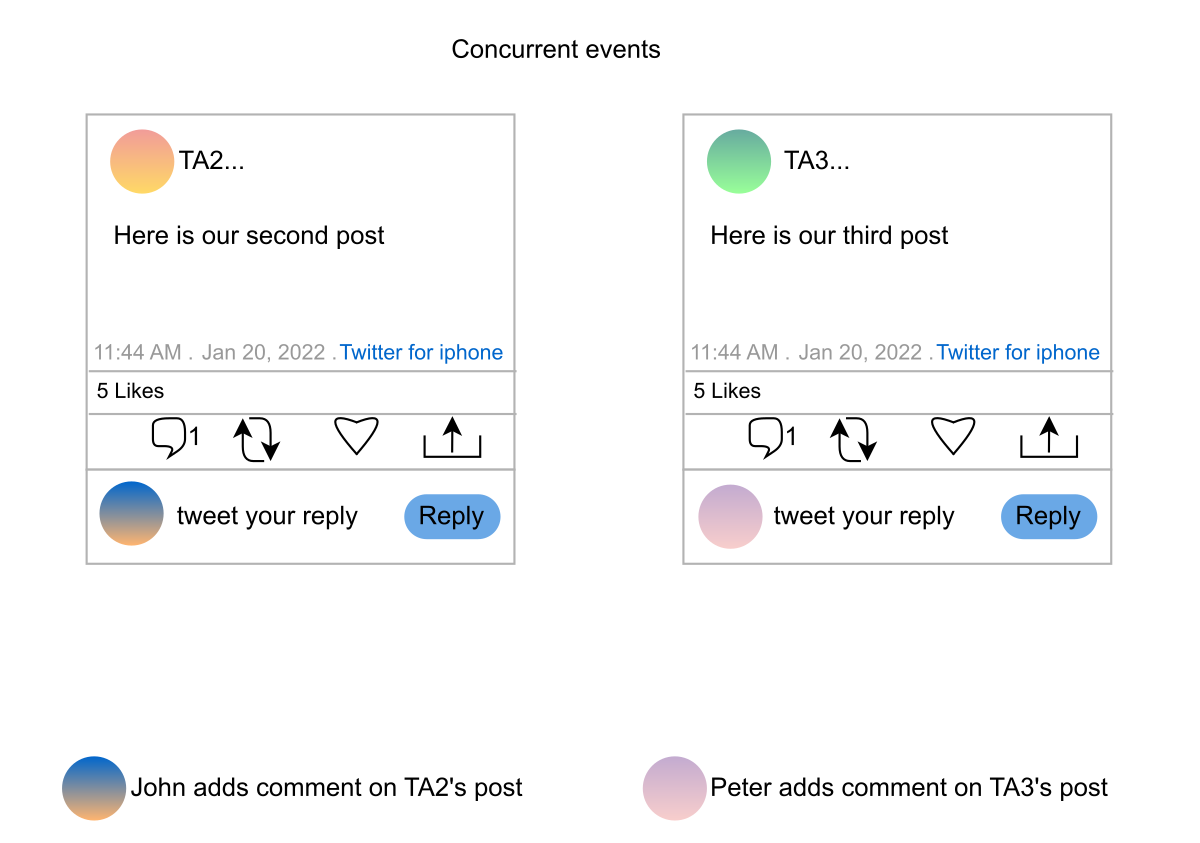
\includegraphics[width=\textwidth]{Images/chapter_12/section_5836711686307840/4942601103081472.png}
 \end{subfigure}
\end{figure}

Some applications need the events to have unique identifiers and carry any relevant causality information. An example of this is giving an identifier to the concurrent writes of a key into a key-value store to implement the last-write-wins strategy.
\\
We can either use logical or physical clocks to infer causality. Some systems have additional requirements where we want event identifiers' causality to map wall-clock time. An example of this is a financial application that complies with the European MiFID regulations. Mi FID requires clocks to be within 100 microseconds of UTC to detect anomalies during high-volume/high-speed market trades.
\begin{quote}
\textbf{Note:} There are many subtleties associated with logical or physical clocks. We can refer to the text below titled ``Time in a Distributed System'' to refresh our concepts of time.
\end{quote}
\\
We use time to determine the sequence of events in our life. For example, if Sam took a bath at 6 a.m. and ate breakfast at 7:00 a.m., we can determine that Sam took a bath before breakfast by the time stamps of each event. Time stamps, therefore, can be used to maintain causality.

\subsubsection{Physical clocks}\label{physical-clocks}
\\
There are often two types of physical clocks available in a computer: the time-of-day clock and monotonic counters.
\\
\paragraph{The time-of-day clock}\label{the-time-of-day-clock}

\begin{itemize}
\tightlist
\item
This usually has lower resolution in comparison to monotonic counters.
\item
Network Time Protocol (NTP) can move the clock forward or backward, so it's not always monotonic.
\item
It may or may not incorporate leap seconds.
\end{itemize}
\\
\paragraph{Monotonic counters}\label{monotonic-counters}

\begin{itemize}
\tightlist
\item
Monotonic counters usually have higher resolution than time-of-day clocks.
\item
Monotonic counters should be used for the duration between two events rather than for the time.
\item
These aren't meaningful across different nodes. For instance, even on the same server with multiple processors, there can be a different counter per processor. The application needs to be careful when using counters from different processors.
\item
The NTP might adjust it without violating monotonicity.
\item
The NTP can only speed up or slow down the counter rate of change by up to 0.05\%.
\end{itemize}

\subsubsection{Reasons for clock drift}\label{reasons-for-clock-drift}
\\
Physical clocks drift over time due to many reasons:

\begin{itemize}
\tightlist
\item
Temperature differences
\item
The equipment's age
\item
Manufacturing defects
\item
Virtualized clocks
\end{itemize}
\\
For instance, a server with a clock drift of 200 parts per million implies a six millisecond drift if synced every 30 seconds, or a 17 seconds drift if re-synced every 24 hours.
\\
A study showed that on the public Internet, an NTP couldn't get clock accuracy better than 35 ms, and it can spike to one second when there's congestion on the network. Otherwise , NTPs use multiple time servers and discards outliers.

\subsubsection{The trade-off: complexity and cost versus clock accuracy}\label{the-trade-off-complexity-and-cost-versus-clock-accuracy}
\\
It's possible to keep clock drift consistently small using GPS and atomic clocks, careful deployment, and monitoring. However, such a system comes with an added dollar cost, as well as increased system complexity.

\subsubsection{Logical clocks}\label{logical-clocks}

\begin{itemize}
\tightlist
\item
Lamport clocks provide us with happened-before relationships. If event A happens before event B, then the clock value of A will be less than the clock value of B. There 's a subtle point that given any two clock values of two events from any two servers, we can't compare them to infer the happened-before relationship because those two events can be concurrent (meaning not causally related).
\item
We can use vector clocks to infer the happened-before relationships using the clock values. For this, we'll need a counter per participating entity in the vector.
\item
We should note that happened-before might not mean that two events were causally related. It might be the case that one event happened before the other. Usually , we need application-level context on top of the happened-before mechanism to infer real causality.
\end{itemize}

\subsection{Use UNIX time stamps}\label{y4Lwdr0G_ewq8N2Bc7kKB}
\\
UNIX time stamps are granular to the millisecond and can be used to distinguish different events. We have an \textbf{ID-generating server} that can generate one ID in a single millisecond. Any request to generate a unique ID is routed to that server, which returns a timestamp and then returns a unique ID. The ability to generate an ID in milliseconds allows us to generate a thousand identifiers per second. This means we can get \protect\phantomsection\label{katex_inline_0gqG4w1ttqL-fCjZNsZnS}{{{\(24 \ (\text{hour}) \times 60 \ (\text{min/hour}) \times 60 \ (\text{sec/min}) \times 1000 \ (\text{ID/sec}) = 86{,}400{,}000 \ \text{IDs}\)}}} in a day. That's less than a billion per day.
\begin{quote}
\textbf{Note:} Connect to the following terminal to view the UNIX time stamp in milliseconds.
\end{quote}

Our system works well with generating IDs, but it poses a crucial problem. The ID-generating server is a single point of failure (SPOF), and we need to handle it. To cater to SPOF, we can add more servers. Each server generates a unique ID for every millisecond. To make the overall identifier unique across the system, we attach the server ID with the UNIX time stamp. Then
, we add a load balancer to distribute the traffic more efficiently. The design of a unique ID generator using a UNIX time stamps is given below:

\begin{figure}[htbp]
 \centering
 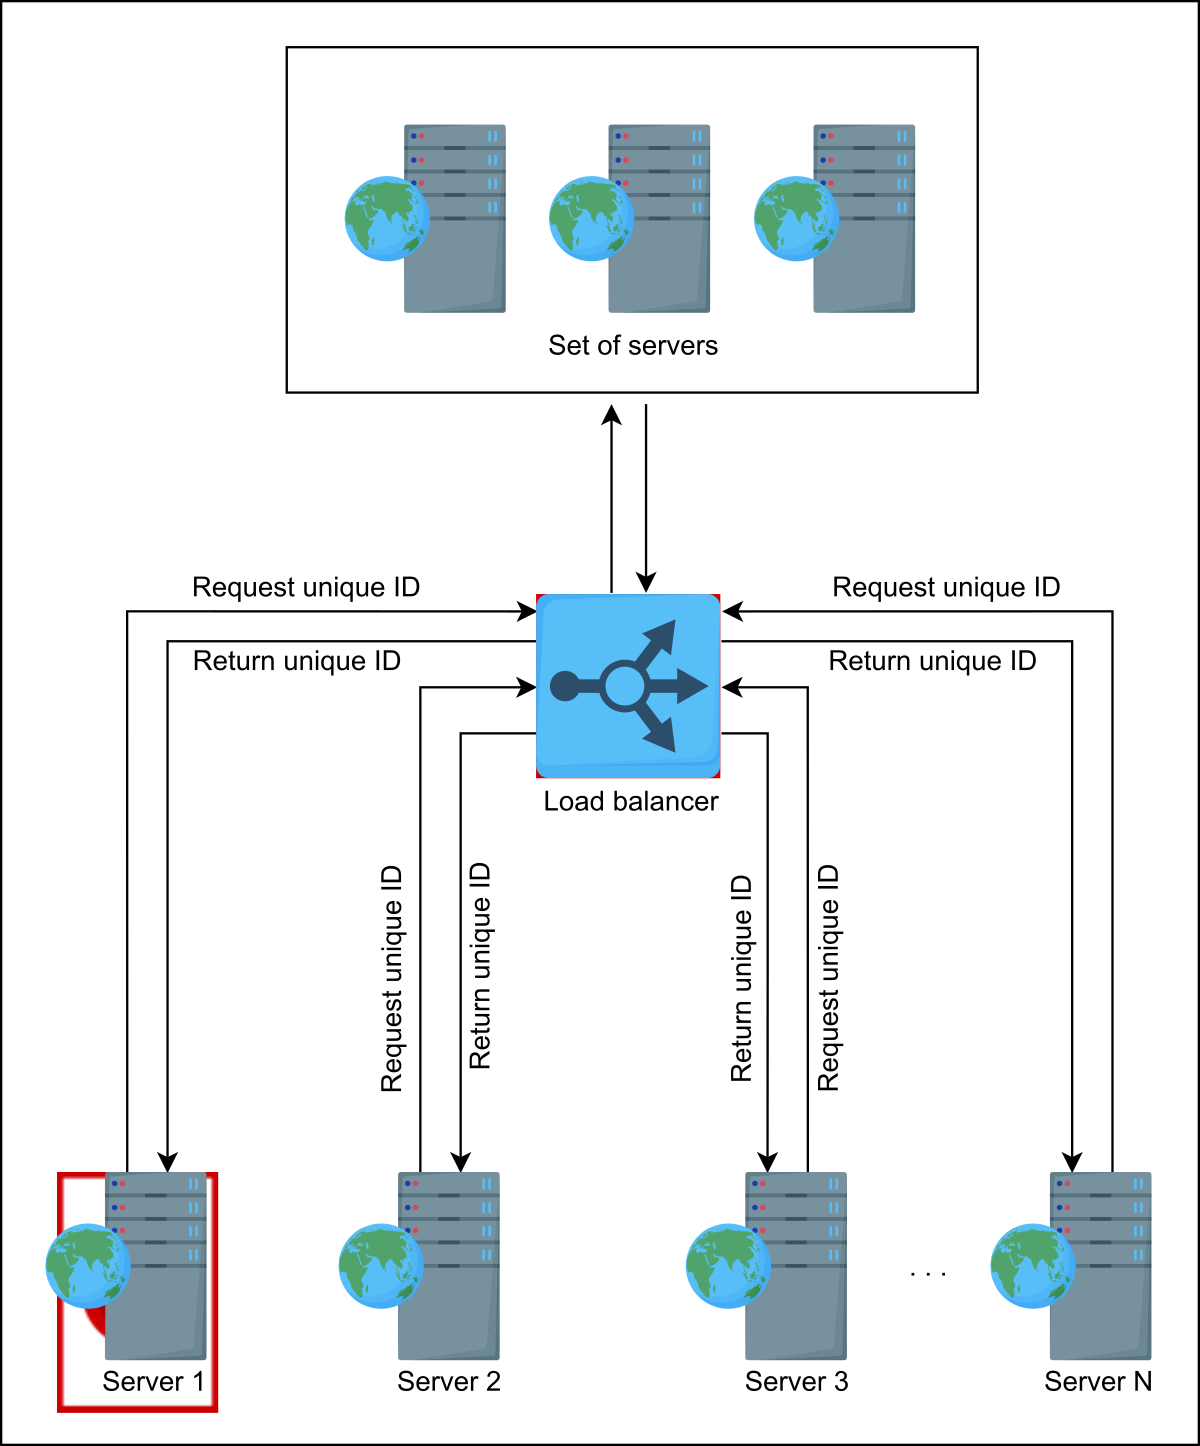
\includegraphics[width=0.5\textwidth]{Images/chapter_12/section_5836711686307840/6638012182429696.png}
 \caption{Using the time stamp as an ID}
\end{figure}

\subsubsection{Pros}\label{81DVK0rSlAhqp5tYpHBXt}
\\
This approach is simple, scalable, and easy to implement. It also enables multiple servers to handle concurrent requests.

\subsubsection{Cons}\label{UojqfrrW1Zz2Sfzd5YApx}
\\
For two concurrent events, the same time stamp is returned and the same ID can be assigned to them. This way, the IDs are no longer unique.

\textbf{Requirements Fulfilled by Each Approach}

\begin{table}[htbp]
\centering
\small
\adjustbox{max width=\textwidth}{
\begin{tabular}{|p{0.230\textwidth}|p{0.124\textwidth}|p{0.114\textwidth}|p{0.100\textwidth}|p{0.177\textwidth}|p{0.205\textwidth}|}
\hline
\hfill\break & \textbf{Unique} & \textbf{Sca{} lable} & \textbf{Available} & \textbf{64-bit numeric ID} & \textbf{Causality maintained} \\
\hline
\hline
\textbf{Using UUID} & no & yes & yes & no & no \\
\hline
\textbf{Using a database} & no & no & yes & yes & no \\
\hline
\textbf{Using a range handler} & yes & yes & yes & yes & no \\
\hline
\textbf{Using UNIX time stamps} & no & \textbf{weak} & yes & yes & \textbf{weak} \\
\hline
\end{tabular}
}
\caption{Requirements Fulfilled by Each Approach}
\end{table}

\subsection{Twitter Snowflake}\label{8geJU6YJN3M77EaZkcYE8}
\\
Let's try to use time efficiently. We can use some bits out of our targetted 64 bits for storing time and the remaining for other information. An overview of division is below:

\begin{figure}[htbp]
 \centering
 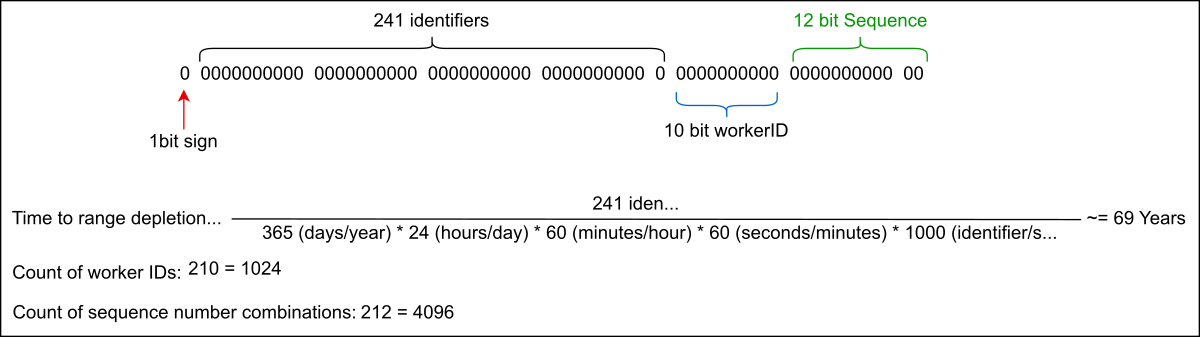
\includegraphics[width=0.5\textwidth]{Images/chapter_12/section_5836711686307840/4912916595998720.png}
 \caption{Overview of the division of bits in Twitter Snowflake}
\end{figure}

The explanation of the bits division is as follows:

\begin{itemize}
\item
\protect\phantomsection\label{lmDQEg2UN7nCZCHjEjBQR}
\textbf{Sign bit}: A single bit is assigned as a sign bit, and its value will always be zero. It makes the overall number positive. Doing so helps to ensure that any programming environment using these identifiers interprets them as positive integers.
\item
\protect\phantomsection\label{R72x9rYoN69BLCHXap141}
\textbf{Time stamp}: 41 bits are assigned for milliseconds. The Twitter Snowflake default epoch will be used. Its value is \protect\phantomsection\label{katex_inline_nmStsr63RDIguzRv7oBMr}{{{\(\text{1288834974657}\)}}}, which is equivalent to November 4, 2010, 01:42:54 UTC. We can initiate our own epoch when our system will be deployed, say January 1, 2022, at 12 midnight can be the start of our epoch from zero. The maximum time to deplete this range is shown below:
\end{itemize}

\[
\text{Time to range depletion} = \frac{2^{41}}{365 \times 24 \times 60 \times 60 \times 1000 } \approx \text{69 years}
\]

The above calculations give us 69 years before we need a new algorithm to generate IDs. As we saw earlier, if we can generate 1,000 identifiers per second, we aren't able to get our target of a billion identifiers per day. Though now, in the Snowflake proposal, we have ample identifiers available when we utilize worker ID and machine local sequence numbers.

\begin{itemize}
\item
\protect\phantomsection\label{LaZdXlLY-0lgVRIrauEi5}
\textbf{Worker number}: The worker number is 10 bits. It gives us \protect\phantomsection\label{katex_inline_gPwgQQP5pDZKEgRIU-rGQ}{{{\(2^{10}\)}}} = 1,024 worker IDs. The server creating the unique ID for its events will attach its ID.
\item
\protect\phantomsection\label{2BSqV1PP6loMdH9do6Z2U}
\textbf{Sequence number}: The sequence number is 12 bits. For every ID generated on the server, the sequence number is incremented by one. It gives us \protect\phantomsection\label{katex_inline_2ZShQKX089XukAaT54Ljr}{{{\(2^{12} = 4,096\)}}} unique sequence numbers. We'll reset it to zero when it reaches 4,096. This number adds a layer to avoid duplication.
\end{itemize}
\\
How can we ensure uniqueness in ID generation when a machine is hit with more than 4,096 requests within the same millisecond, given that the sequence number in the ID structure ensures uniqueness within the same millisecond?
\\
Use the AI assessment widget below to submit your solution and get an interactive response.

\textbf{Question:}

What happens if the ID limit is exceeded?

\textbf{Reference Answer:}

If a machine tries to generate more than 4,096 IDs in one millisecond, it waits for the next millisecond to continue. This adds a tiny delay, but in practice, the wait is so short that it rarely impacts performance. Most systems don't hit this limit under normal workloads.

The following slides show the conversion of the time stamp to UTC.

\begin{figure}[htbp]
 \centering
 \begin{subfigure}[b]{0.48\textwidth}
 \centering
 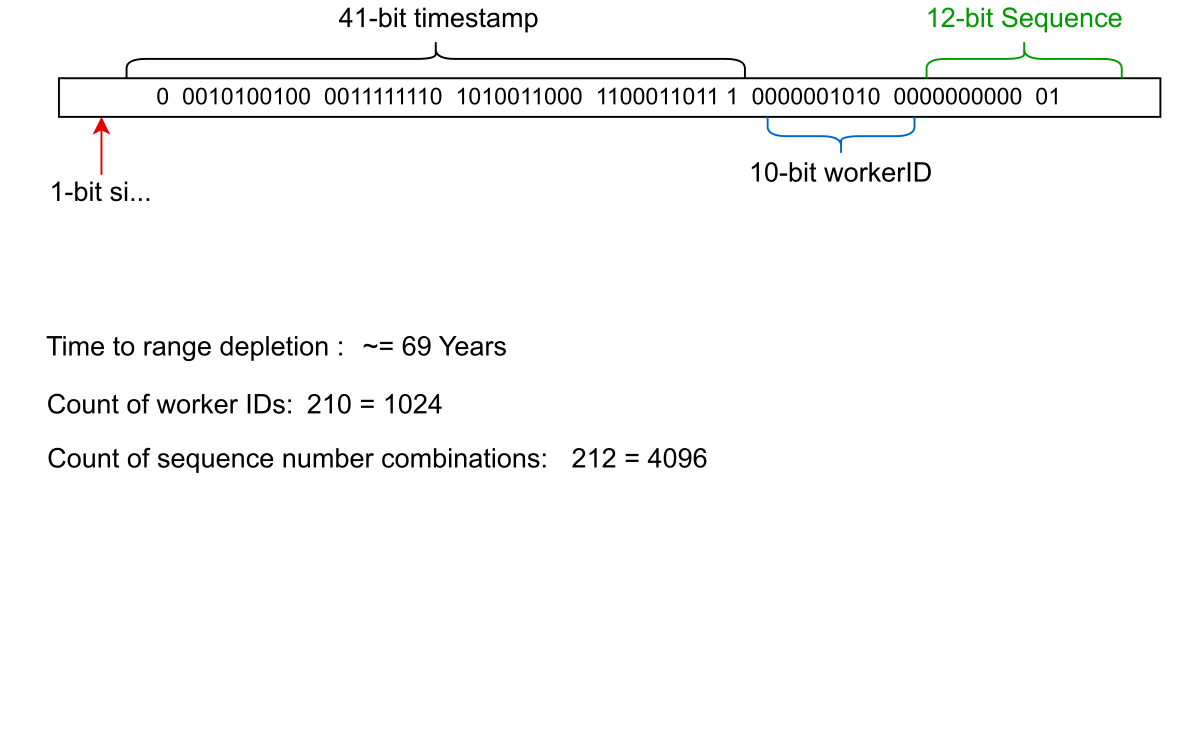
\includegraphics[width=\textwidth]{Images/chapter_12/section_5836711686307840/5204381729554432.png}
 \caption{Overview of the division of bits}
 \end{subfigure}
 \hfill
 \begin{subfigure}[b]{0.48\textwidth}
 \centering
 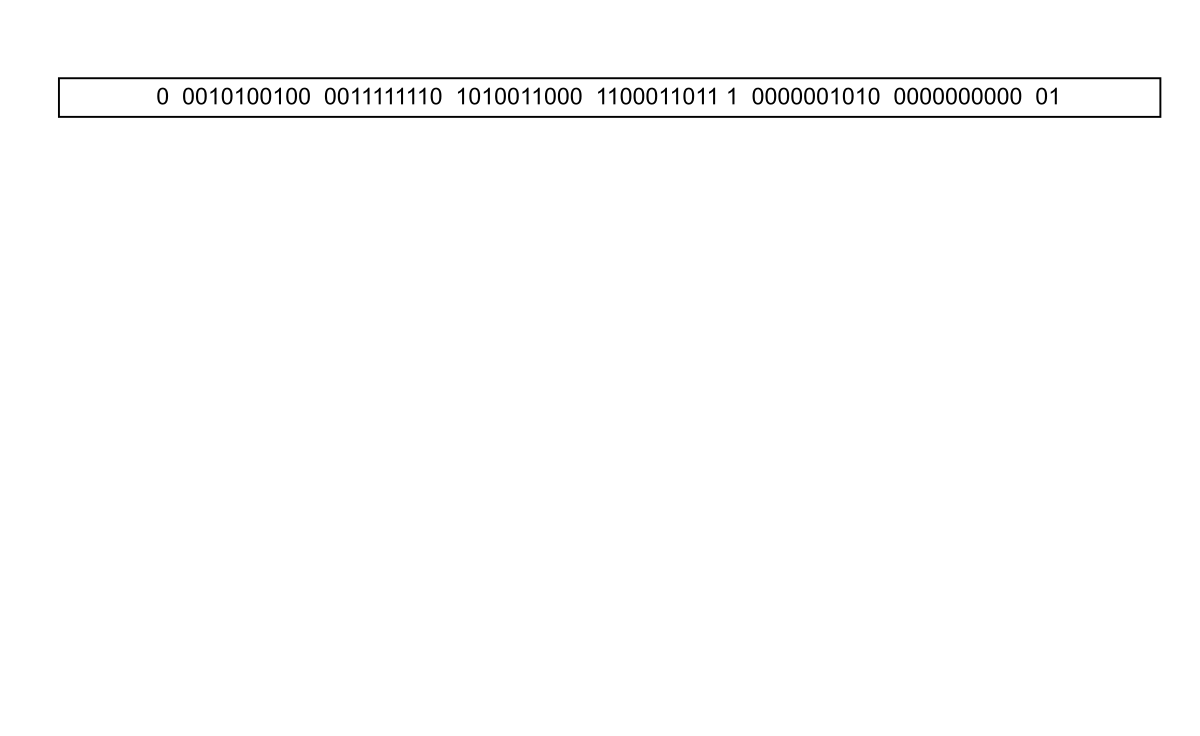
\includegraphics[width=\textwidth]{Images/chapter_12/section_5836711686307840/6042422076768256.png}
 \caption{Convert the time to UTC}
 \end{subfigure}
\end{figure}

\begin{figure}[htbp]
 \centering
 \begin{subfigure}[b]{0.48\textwidth}
 \centering
 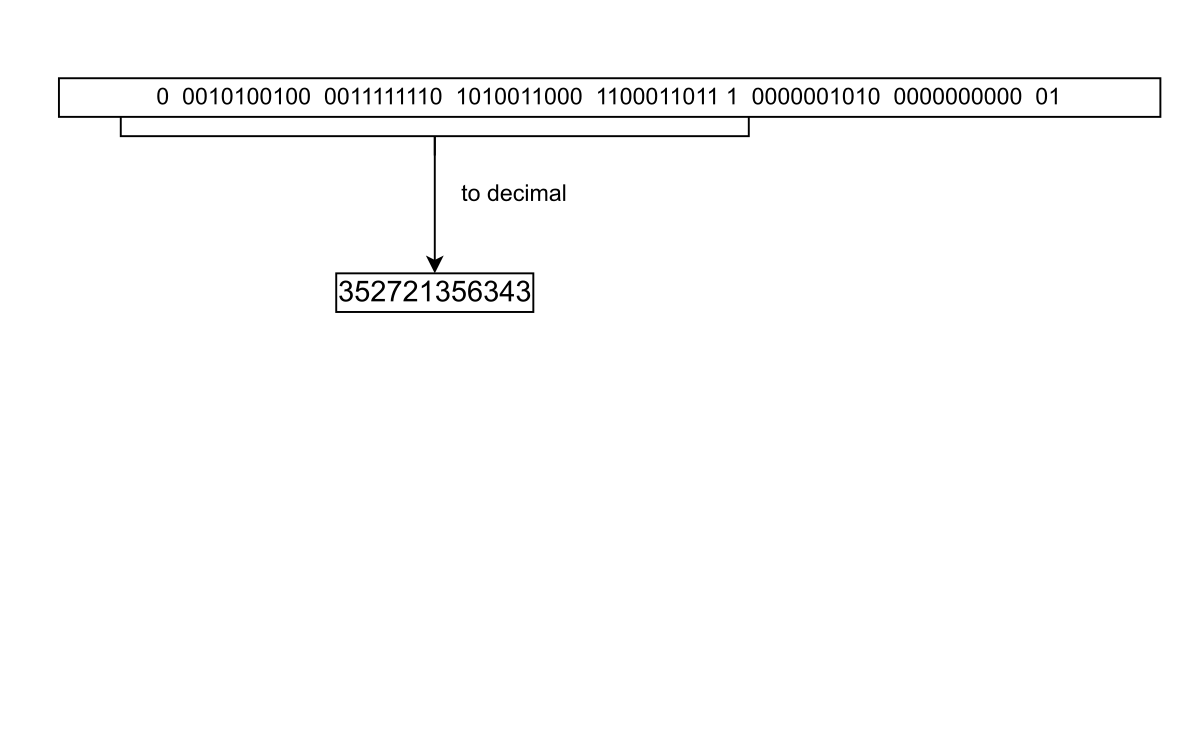
\includegraphics[width=\textwidth]{Images/chapter_12/section_5836711686307840/6377370503610368.png}
 \caption{Convert the bits to decimal}
 \end{subfigure}
 \hfill
 \begin{subfigure}[b]{0.48\textwidth}
 \centering
 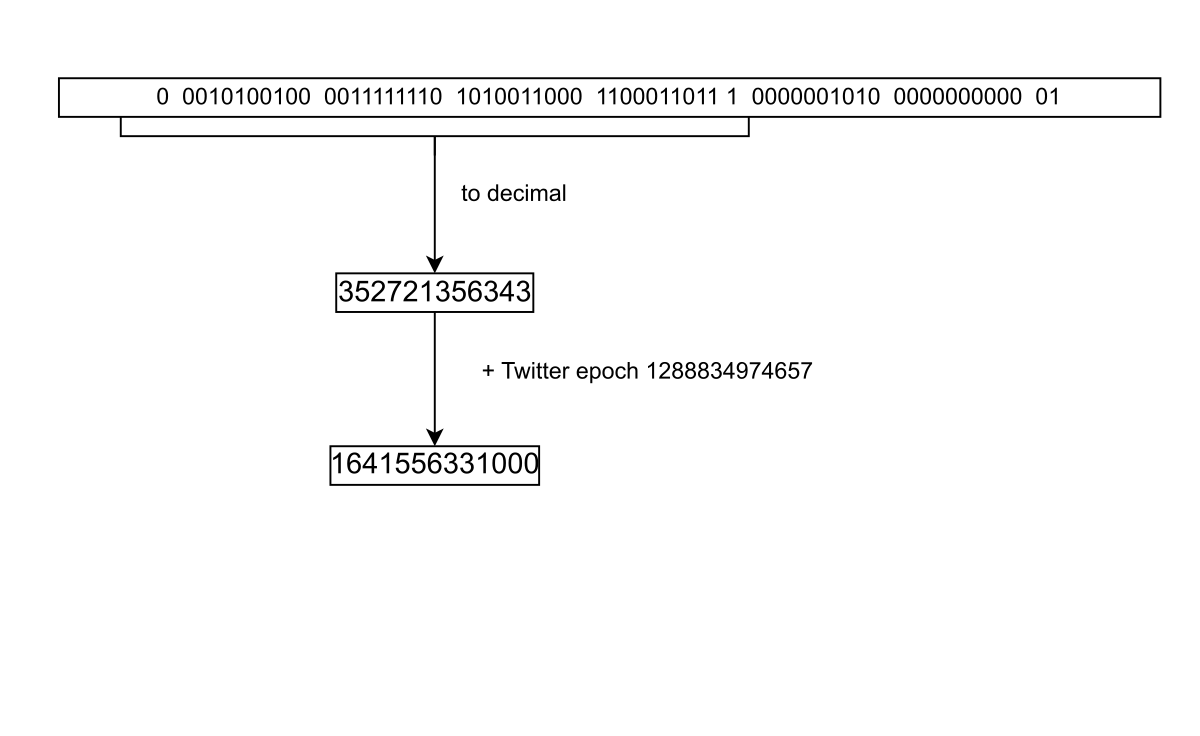
\includegraphics[width=\textwidth]{Images/chapter_12/section_5836711686307840/5870811054866432.png}
 \caption{Convert the decimal to epoch}
 \end{subfigure}
\end{figure}

\begin{figure}[htbp]
 \centering
 \begin{subfigure}[b]{0.48\textwidth}
 \centering
 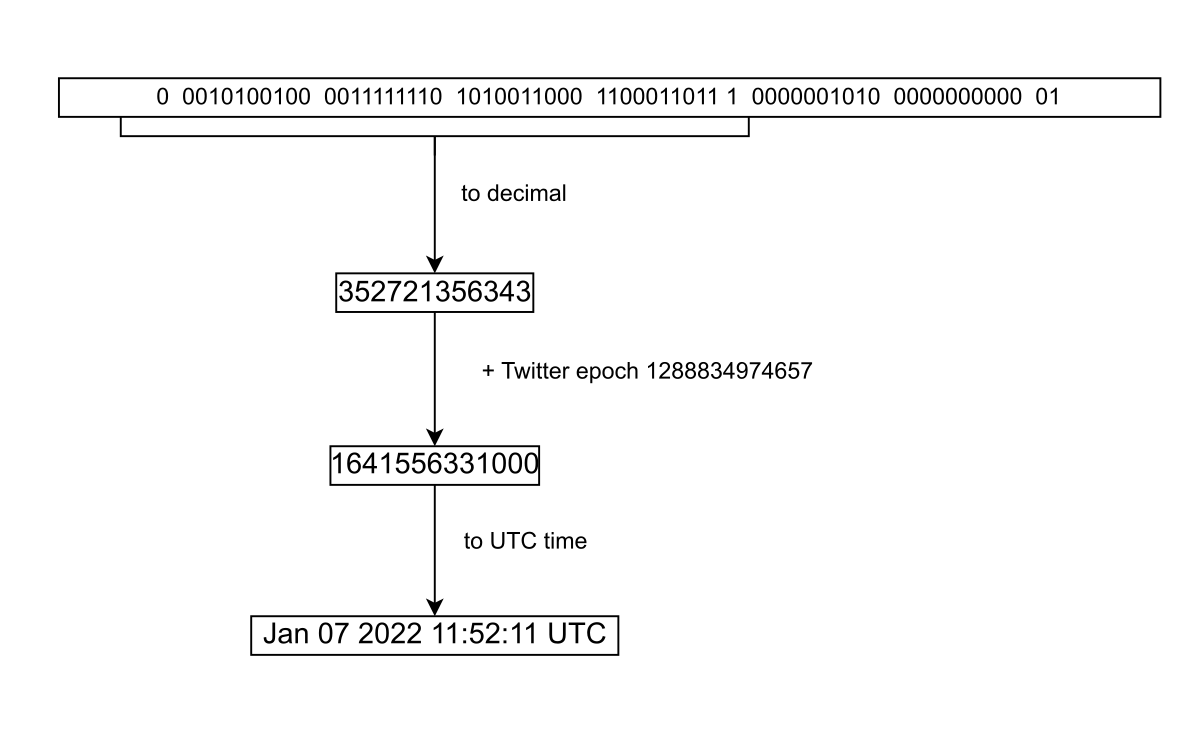
\includegraphics[width=\textwidth]{Images/chapter_12/section_5836711686307840/4825885441523712.png}
 \caption{Convert milliseconds to UTC}
 \end{subfigure}
\end{figure}

\subsubsection{Pros}\label{XHOkiV_chtoqG9L8sVquH}
\\
Twitter Snowflake uses the time stamp as the first component. Therefore, they're time sortable. The ID generator is highly available as well.

\subsubsection{Cons}\label{xRJI_cwu3HNZJOs2fnsHu}
\\
IDs generated in a \textbf{dead period} are a problem. The dead period is when no request for generating an ID is made to the server. These IDs will be wasted since they take up identifier space. The unique range possible will deplete earlier than expected and create gaps in our global set of user IDs.

\begin{quote}
\textbf{Quiz:}
\textbf{Question 1:} Can you find another shortcoming in the design shown above?
\textbf{Answer:} The  physical clocks: A device used to measure and indicate time,

e.g., pendulums, hourglass, quartz clock, etc.  are unreliable.

For such clocks, the error can be 17 seconds per day. If we measure time using these on a server, the time drifts away. Considering a single server, we won\textquotesingle t be affected by the drifting away of time since all transactions land on a single server. But in a distributed environment, the clocks won\textquotesingle t remain synced.

Due to the unreliability of measuring accurate time, no matter how often we synchronize these clocks with each other or other clocks with accurate measurement methods, there will always be \_skew\_ between the various clocks involved in a distributed system.
\end{quote}

Another weak point of this system is its reliance on time. NTP can affect the working of this system. If the clock on one of the servers drifts two seconds in the future, other servers are two seconds behind. The NTP clock recognizes it and recalibrates its clock. Now, all serves will be aligned. However, in that drifting process, IDs could have been generated for a time that hasn't occurred yet, and now we'll have a pair of possible nonconcurrent events with the same time stamp. Lastly
, the causality of our events won't be maintained.
\begin{quote}
\textbf{Note:} The Network Time Protocol (NTP) is a networking protocol for clock synchronization between computer systems over packet-switched, variable-latency data networks. NTP intends to synchronize all participating computers within a few milliseconds of Coordinated Universal Time (UTC). It mitigates the effects of variable network latency.
\end{quote}
\\
Having accurate time still remains an issue. We can read a machine's time-of-day clock with microsecond or even nanosecond resolution. Even with this fine-grained measurement, the risks of NTP(NTP servers can be susceptible to man-in-the-middle attacks unless packets are cryptographically signed for authentication. The computational overhead involved can make this impractical on busy servers, particularly during denial of service attacks. NTP message spoofing from a man-in-the-middle attack can be used to move clocks on client computers and allow several attacks based on bypassing cryptographic key expiration. Some of the services affected by fake NTP messages identified are TLS, DNSSEC, various caching schemes (such as DNS cache), BGP, Bitcoin, and many persistent login schemes.)remain. Since we can't rely on physical clocks, let's put logical clocks to use.
\\
The following table gives an overview of the requirements that have been fulfilled using different design approaches.

\textbf{Requirements Fulfilled by Each Approach}

\begin{table}[htbp]
\centering
\small
\adjustbox{max width=\textwidth}{
\begin{tabular}{|p{0.230\textwidth}|p{0.124\textwidth}|p{0.114\textwidth}|p{0.100\textwidth}|p{0.177\textwidth}|p{0.205\textwidth}|}
\hline
\hfill\break & \textbf{Unique} & \textbf{Sca{} lable} & \textbf{Available} & \textbf{64-bit numeric ID} & \textbf{Causality maintained} \\
\hline
\hline
\textbf{Using UUID} & no & yes & yes & no & no \\
\hline
\textbf{Using a database} & no & no & yes & yes & no \\
\hline
\textbf{Using a range handler} & yes & yes & yes & yes & no \\
\hline
\textbf{Using UNIX time stamps} & no & \textbf{weak} & yes & yes & \textbf{weak} \\
\hline
\textbf{Using Twitter Snowflake} & yes & yes & yes & yes & \textbf{weak} \\
\hline
\end{tabular}
}
\caption{Requirements Fulfilled by Each Approach}
\end{table}

\subsection{Using logical clocks}\label{pzoCD1h8qFHujgeCThCn0}
\\
We can utilize logical clocks (Lamport and vector clocks) that need monotonically increasing identifiers for events.

\subsubsection{Lamport clocks}\label{8CiRv1fmewL4y2Qed65n8}
\\
Lamport clocks are a logical time mechanism used to establish a partial ordering of events in a distributed system. Each process maintains a counter, initialized to zero, which is incremented before every local event. When a process sends a message, it includes its current counter value as a timestamp. Upon receiving a message, the recipient process sets its clock to \protect\phantomsection\label{katex_inline_9LlELwexNdU3UkX21IWZ8}{{{\(\text{max(local clock, received timestamp) + 1}\)}}} before recording the message-receipt event. This mechanism guarantees that if event \texttt{a} causally precedes event \texttt{b}, then the logical timestamp assigned to \texttt{a} will be less than that of \texttt{b}.
\\
Lamport clocks provide a unique partial ordering of events using the happened-before relationship. We can also get a total ordering of events by tagging unique node/process identifiers, though such ordering isn't unique and will change with a different assignment of node identifiers. However, we should note that Lamport clocks don't allow us to infer causality at the global level. This means we can't simply compare two clock values on any server to infer happened-before relationship. Vector clocks overcome this shortcoming.

\subsubsection{Vector clocks}\label{LgHTatjJPt8053_N3B5Sa}
\\
Vector clocks maintain causal history---that is, all information about the happened-before relationships of events. So , we must choose an efficient data structure to capture the causal history of each event.
\\
Consider the design shown below. We 'll generate our ID by concatenating relevant information, just like the Twitter snowflake, with the following division:

\begin{itemize}
\item
\protect\phantomsection\label{qgekgNPlqHdArmD3VB9qM}
\textbf{Sign bit}: A single bit is assigned as a sign bit, and its value will always be zero.
\item
\protect\phantomsection\label{rfFk67ptwoZWkdOLnpjhv}
\textbf{Vector clock}: This is 53 bits and the counters of each node.
\item
\protect\phantomsection\label{hk62wqibjcNZ1_wEP5t-d}
\textbf{Worker number}: This is 10 bits. It gives us \protect\phantomsection\label{katex_inline_83dBy1kuxhnU1YYGSCQKP}{{{\(2^{10} = 1,024\)}}} worker IDs.
\end{itemize}
\\
The following slides explain the unique ID generation using vector clocks, where the nodes A, B, and C reside in a data center.

\begin{quote}
\textbf{Note:} In the following slides, we haven't converted the data to bits for the sake of understanding. The pattern we'll use for the unique ID is the following:

\begin{verbatim}
[vector-clock][worker-id]
\end{verbatim}
\end{quote}

\begin{figure}[htbp]
 \centering
 \begin{subfigure}[b]{0.48\textwidth}
 \centering
 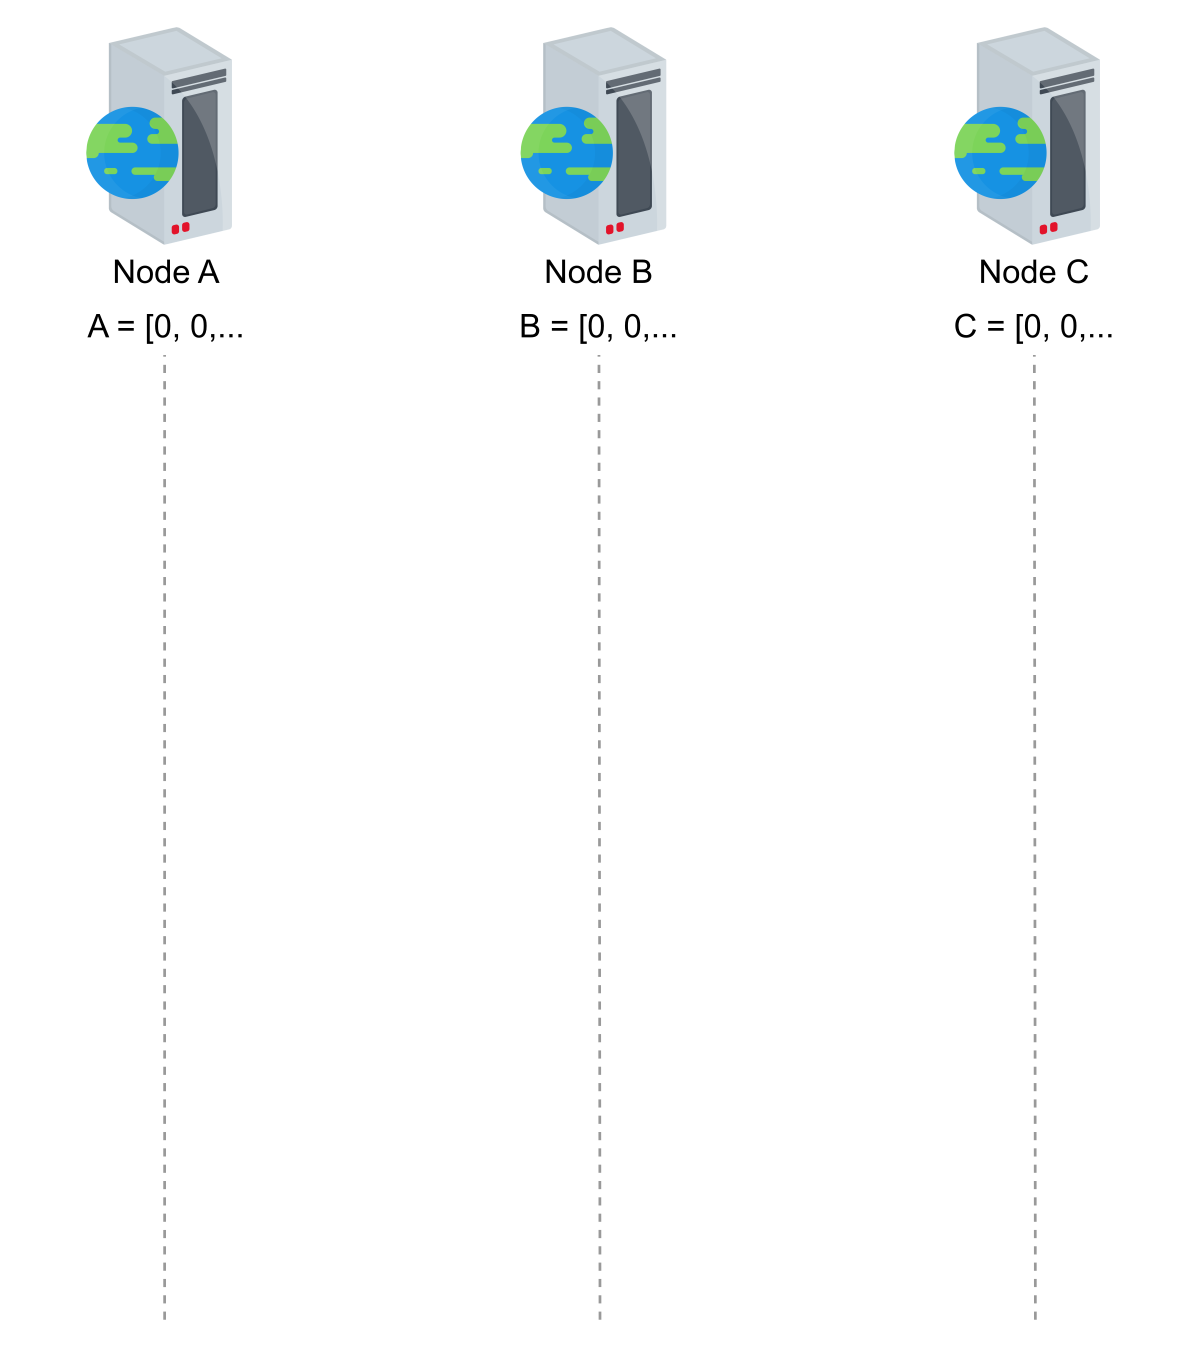
\includegraphics[width=\textwidth]{Images/chapter_12/section_5836711686307840/6037503342411776.png}
 \caption{No event is currently in progress}
 \end{subfigure}
 \hfill
 \begin{subfigure}[b]{0.48\textwidth}
 \centering
 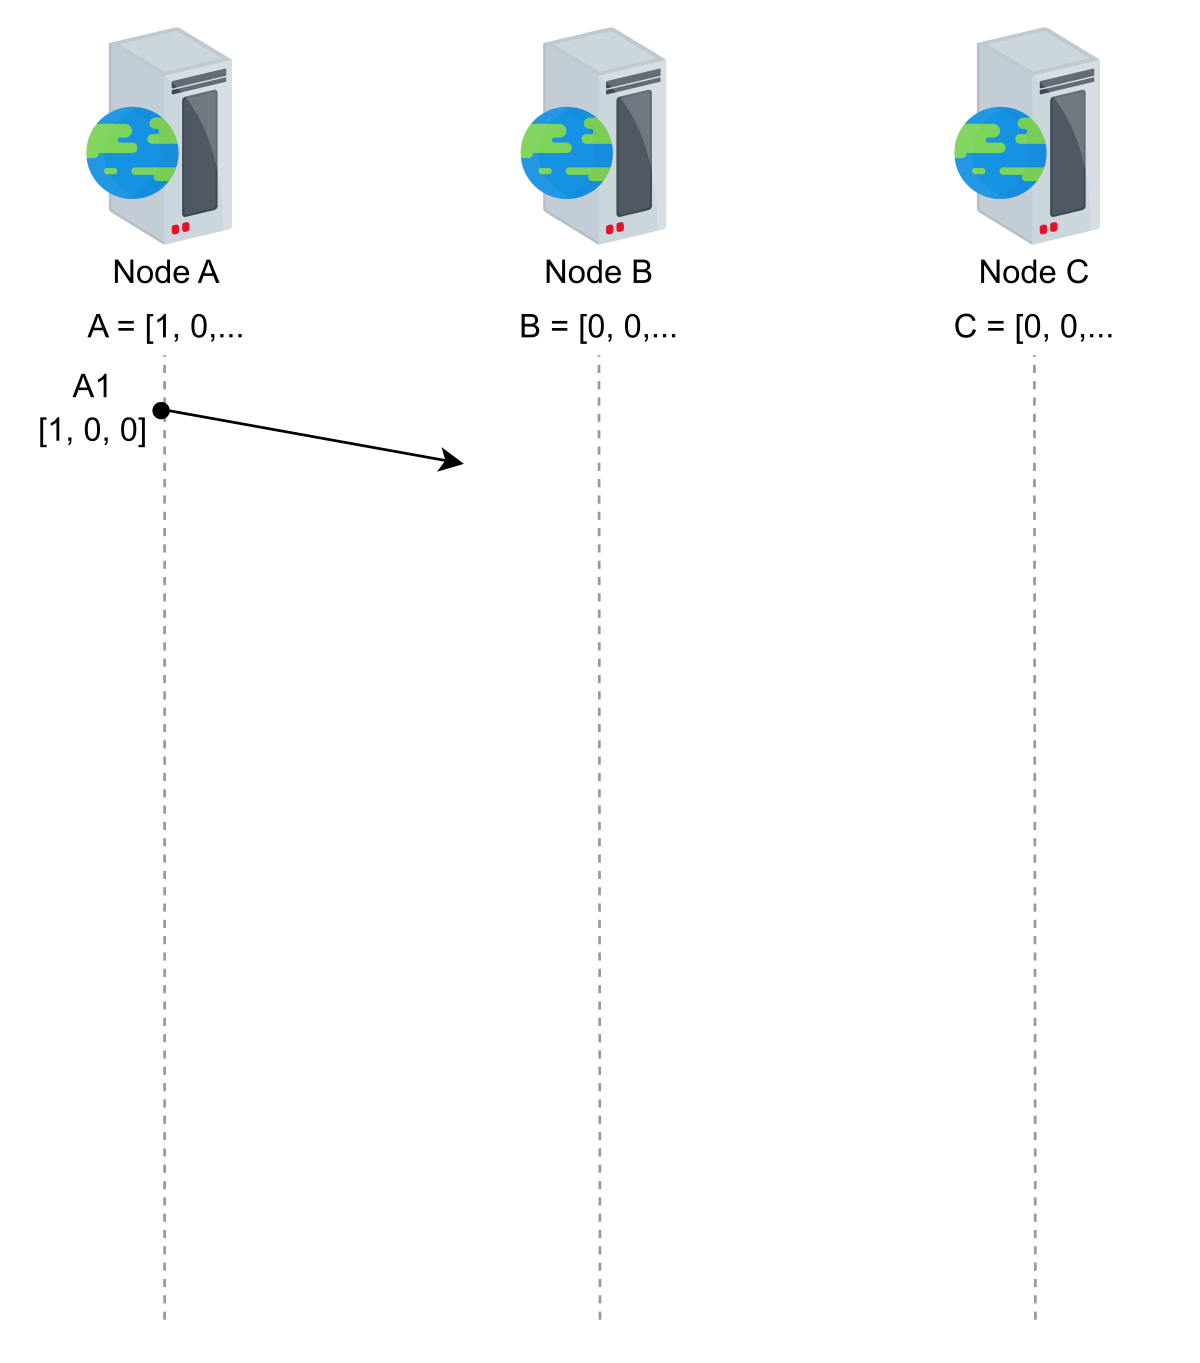
\includegraphics[width=\textwidth]{Images/chapter_12/section_5836711686307840/4809773284196352.png}
 \caption{Unique ID for A1: [1,0,0][A]}
 \end{subfigure}
\end{figure}

\begin{figure}[htbp]
 \centering
 \begin{subfigure}[b]{0.48\textwidth}
 \centering
 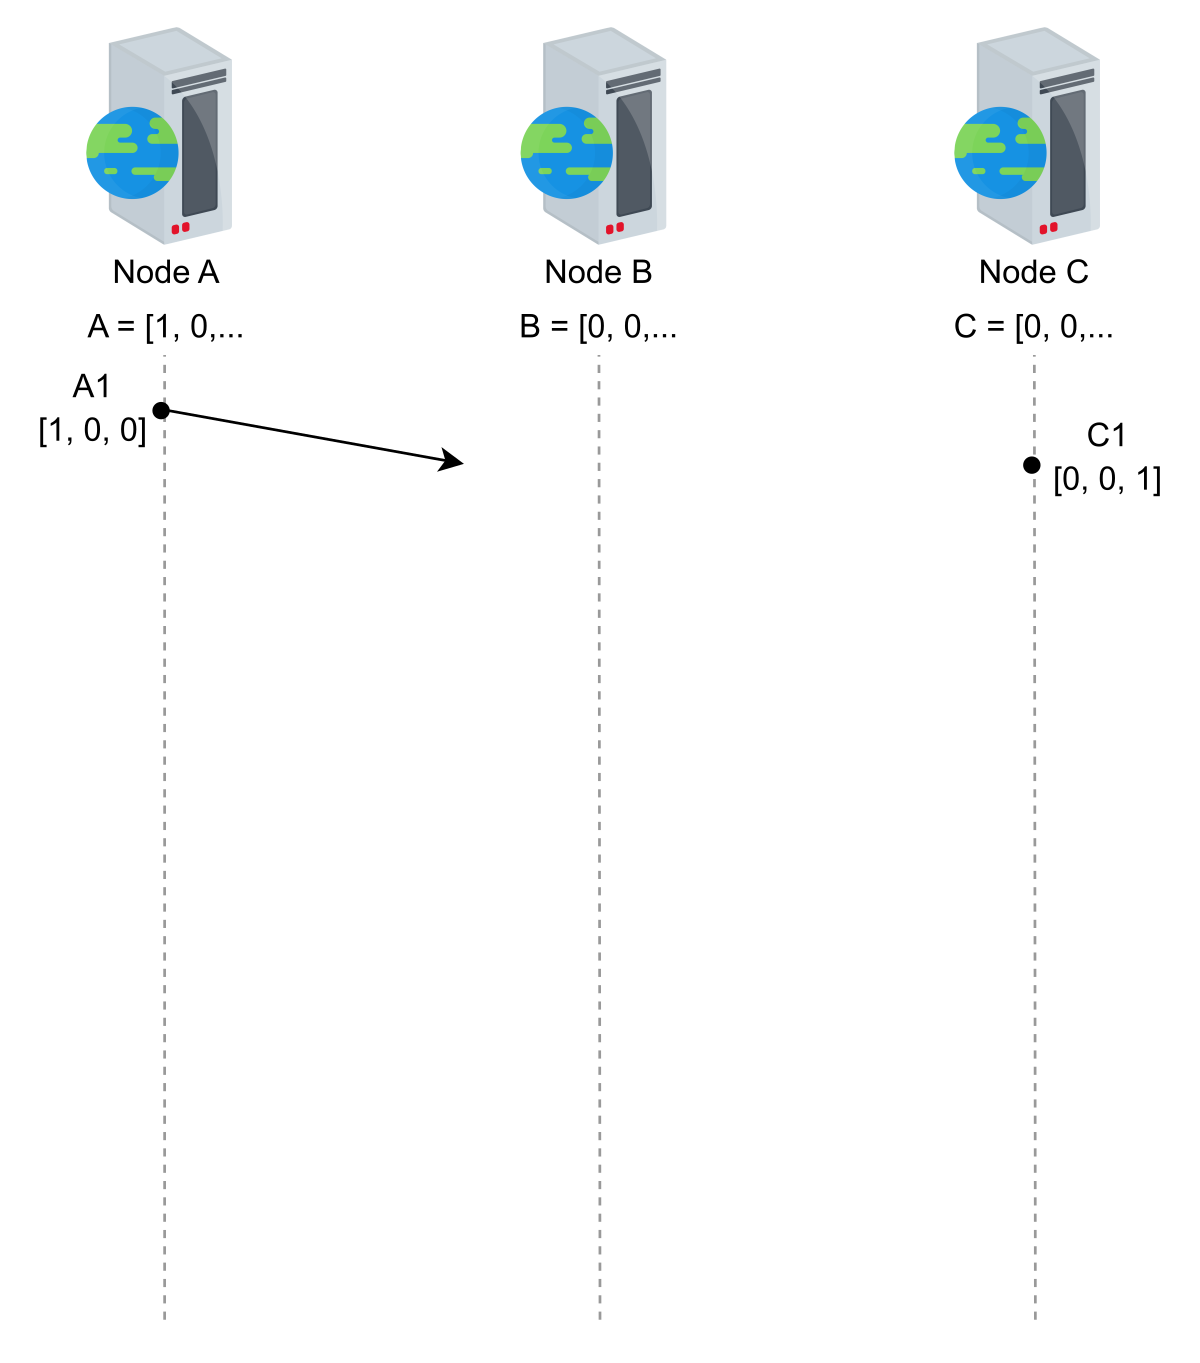
\includegraphics[width=\textwidth]{Images/chapter_12/section_5836711686307840/5107587088252928.png}
 \caption{Unique ID for C1: [0,0,1][C]}
 \end{subfigure}
 \hfill
 \begin{subfigure}[b]{0.48\textwidth}
 \centering
 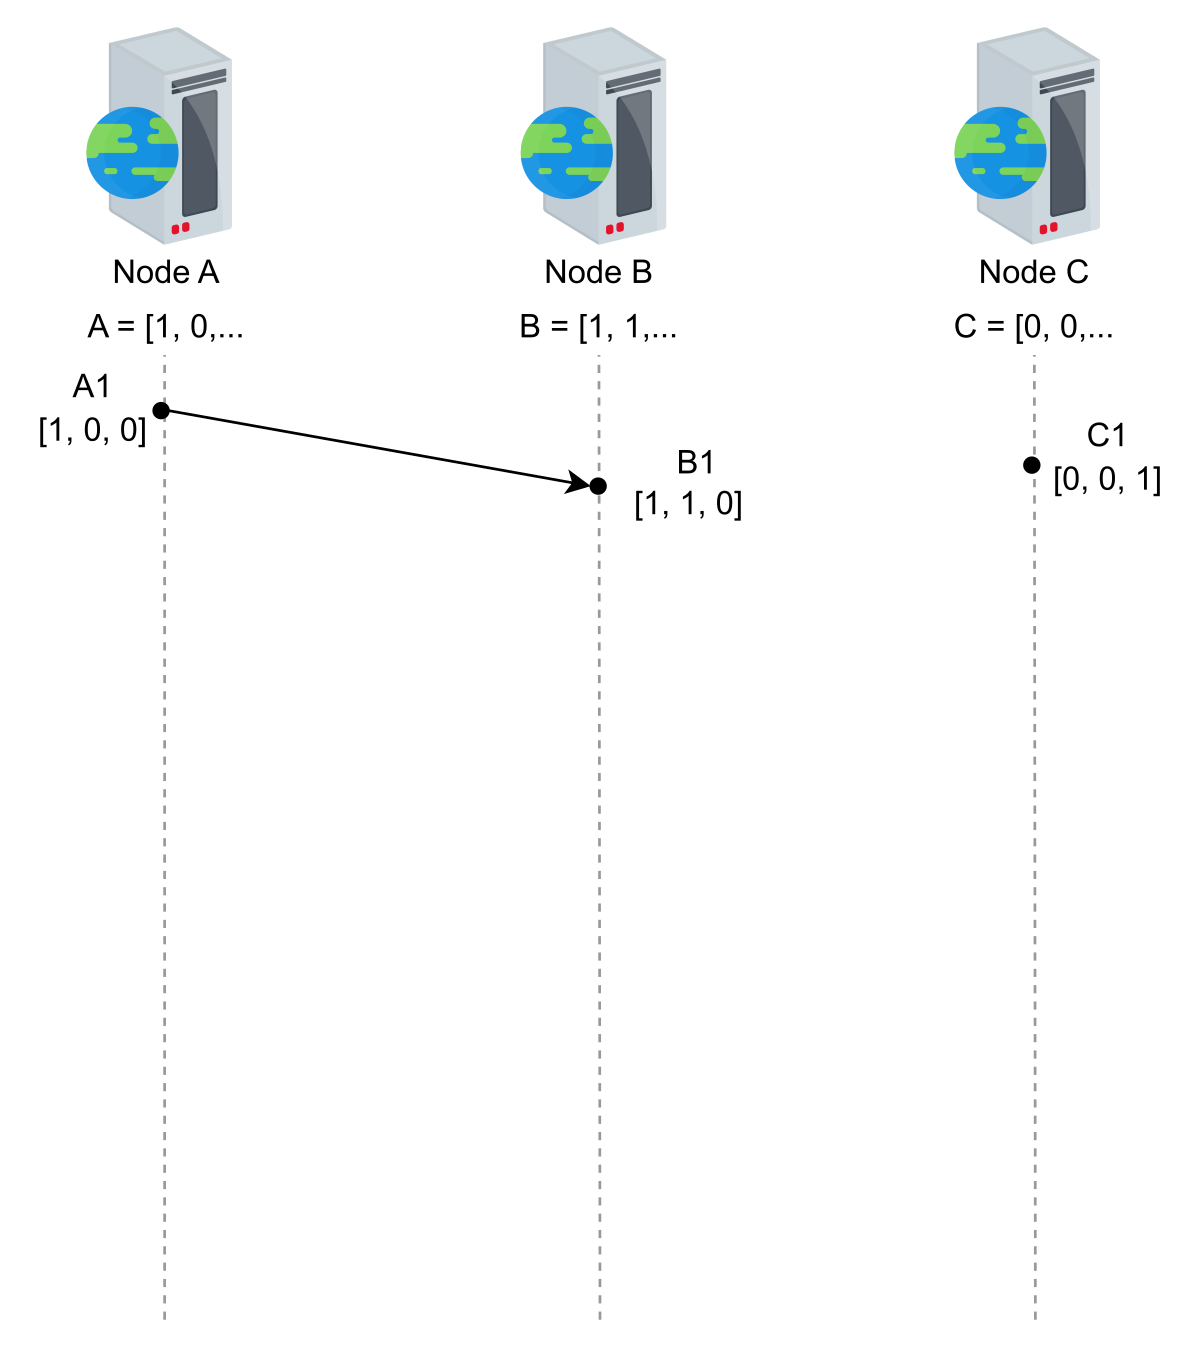
\includegraphics[width=\textwidth]{Images/chapter_12/section_5836711686307840/6176139820007424.png}
 \caption{Unique ID for B1: [1,1,0][B]}
 \end{subfigure}
\end{figure}

\begin{figure}[htbp]
 \centering
 \begin{subfigure}[b]{0.48\textwidth}
 \centering
 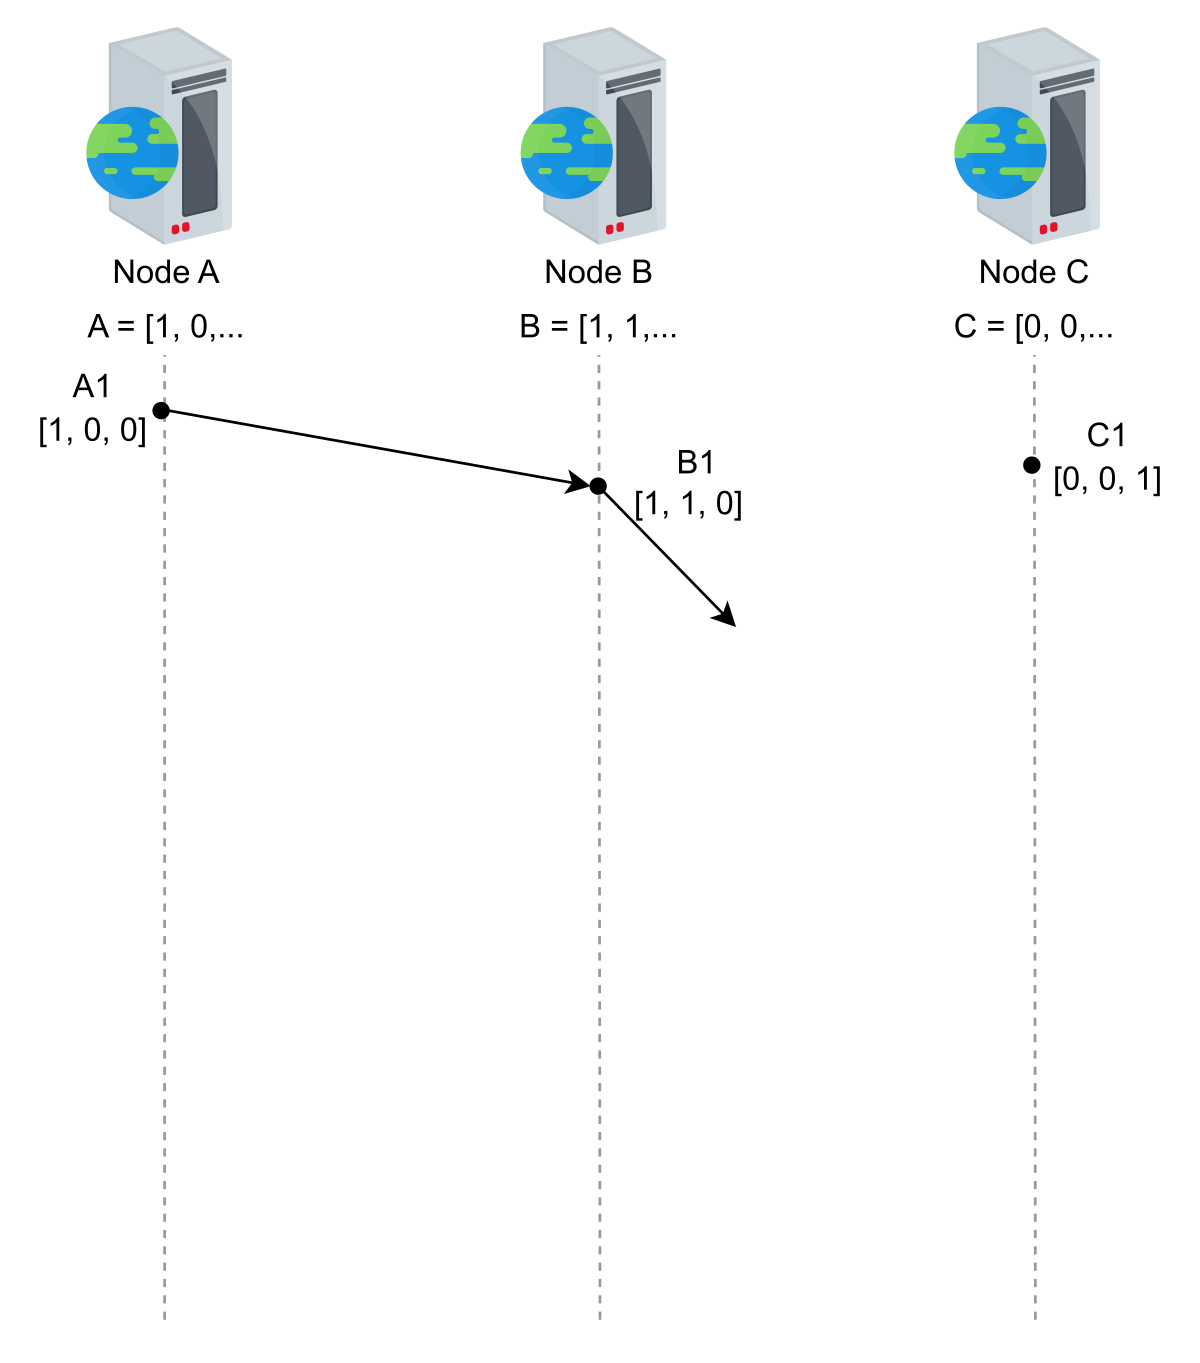
\includegraphics[width=\textwidth]{Images/chapter_12/section_5836711686307840/4846411066507264.png}
 \caption{No new ID needs to be assigned}
 \end{subfigure}
 \hfill
 \begin{subfigure}[b]{0.48\textwidth}
 \centering
 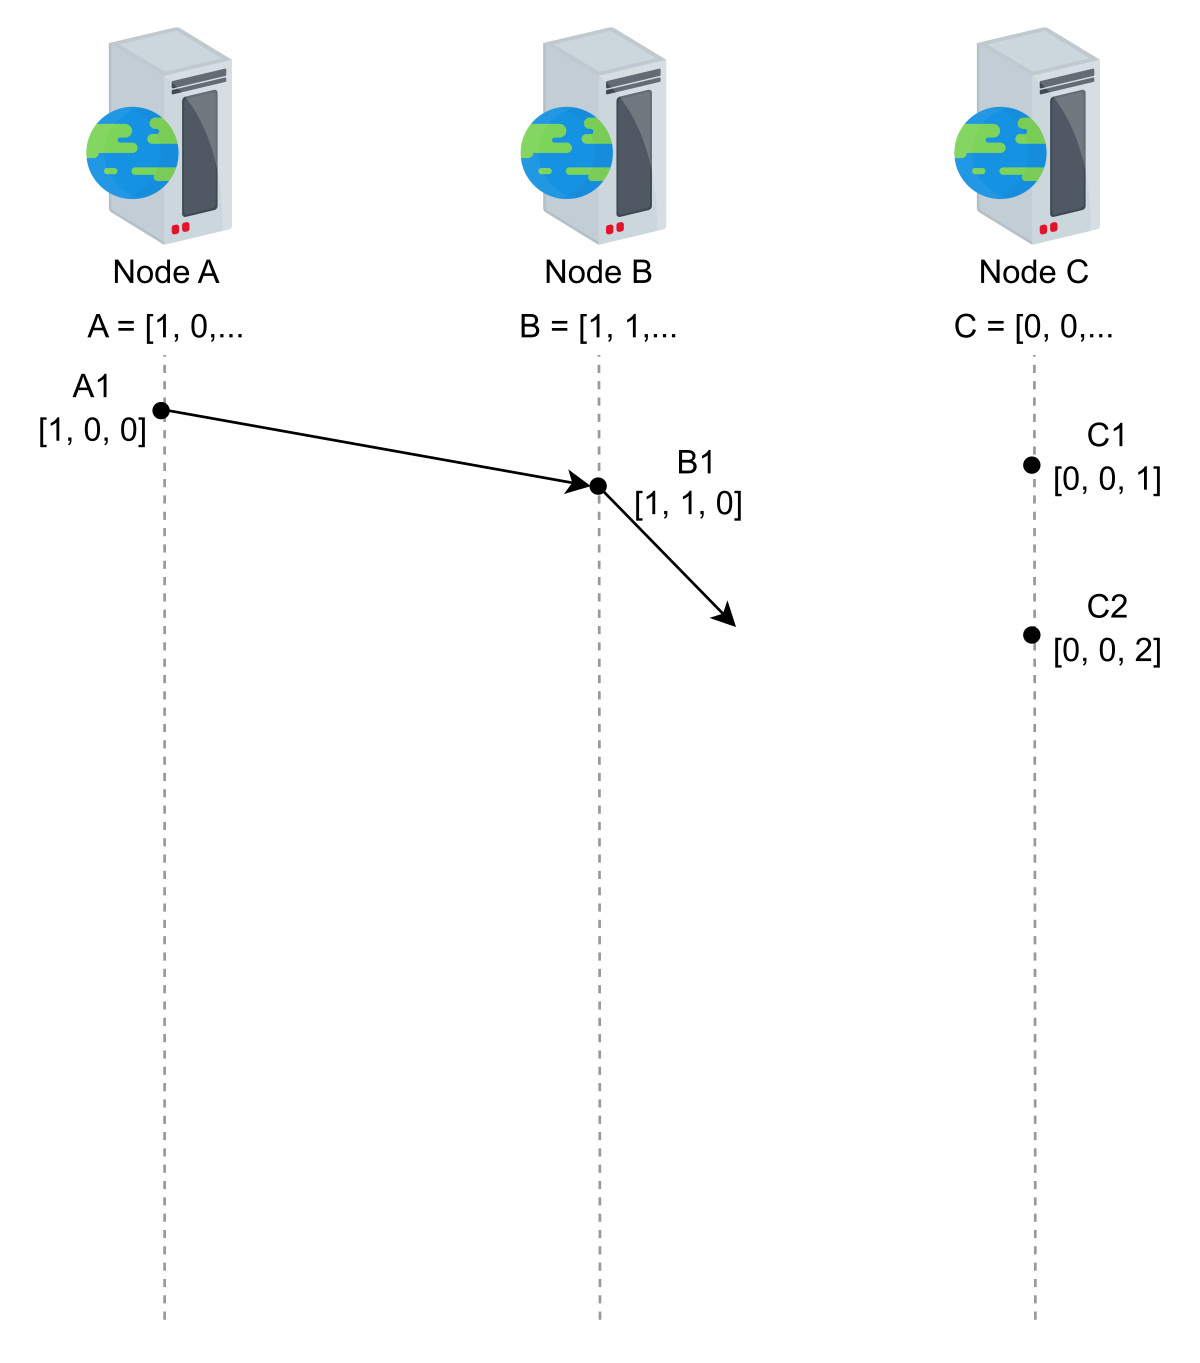
\includegraphics[width=\textwidth]{Images/chapter_12/section_5836711686307840/4800106487218176.png}
 \caption{Unique ID for C2: [0,0,2][C]}
 \end{subfigure}
\end{figure}

\begin{figure}[htbp]
 \centering
 \begin{subfigure}[b]{0.48\textwidth}
 \centering
 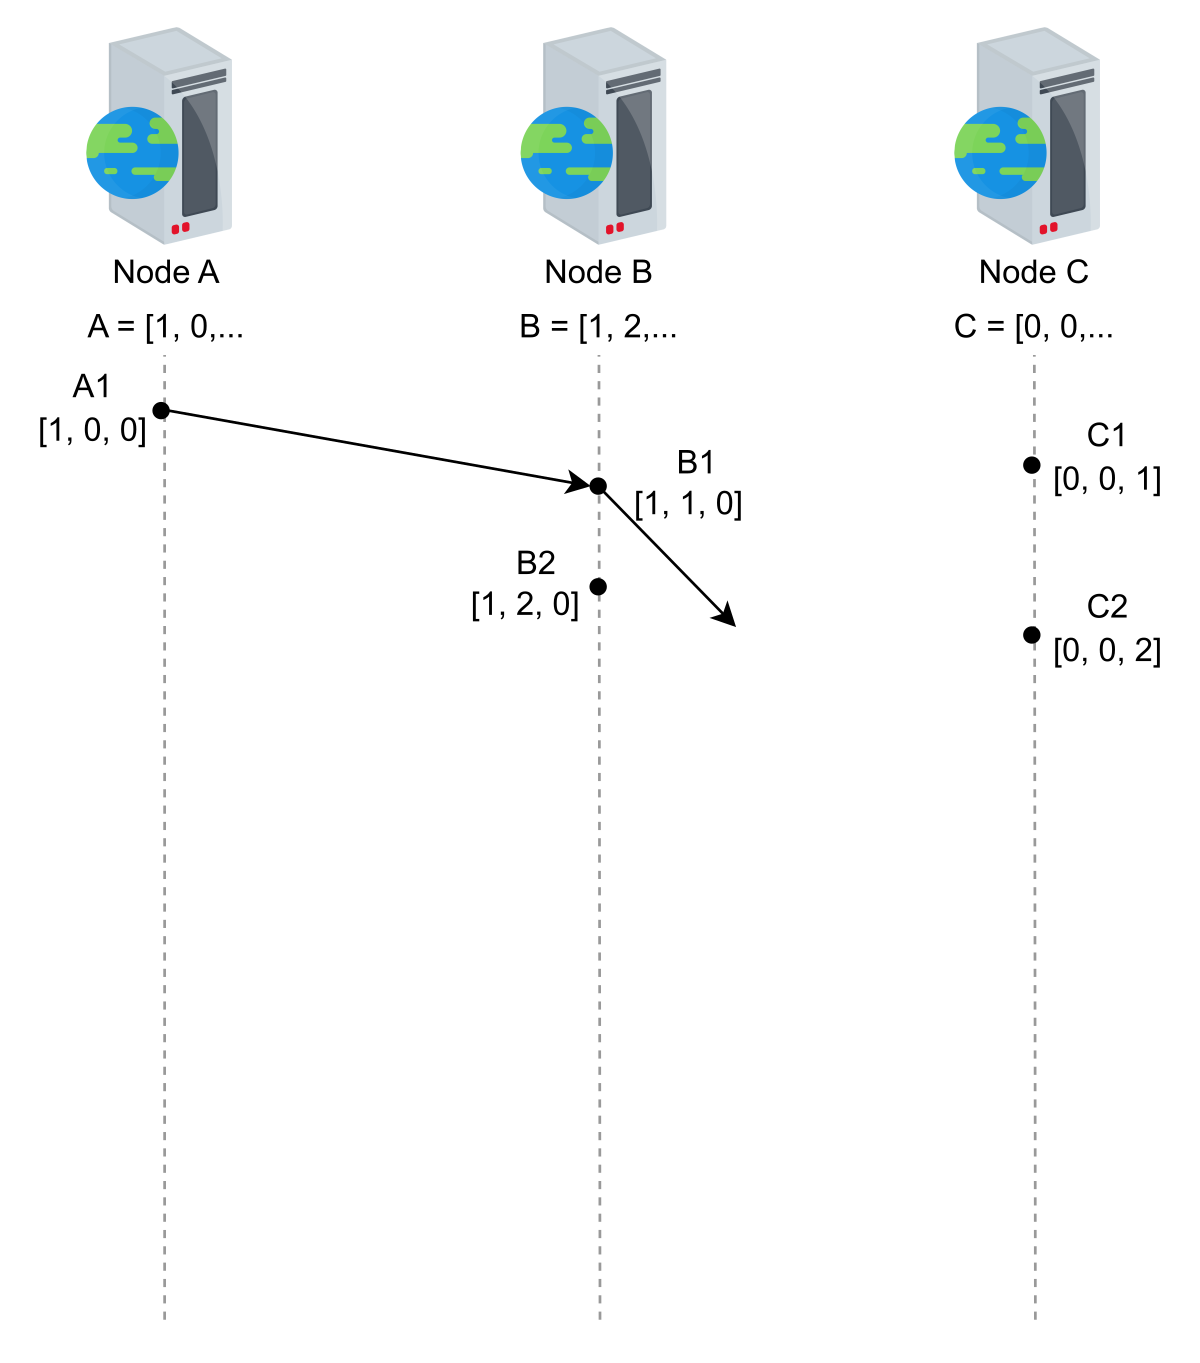
\includegraphics[width=\textwidth]{Images/chapter_12/section_5836711686307840/6298372290772992.png}
 \caption{Unique ID for B2: [1,2,0][B]}
 \end{subfigure}
 \hfill
 \begin{subfigure}[b]{0.48\textwidth}
 \centering
 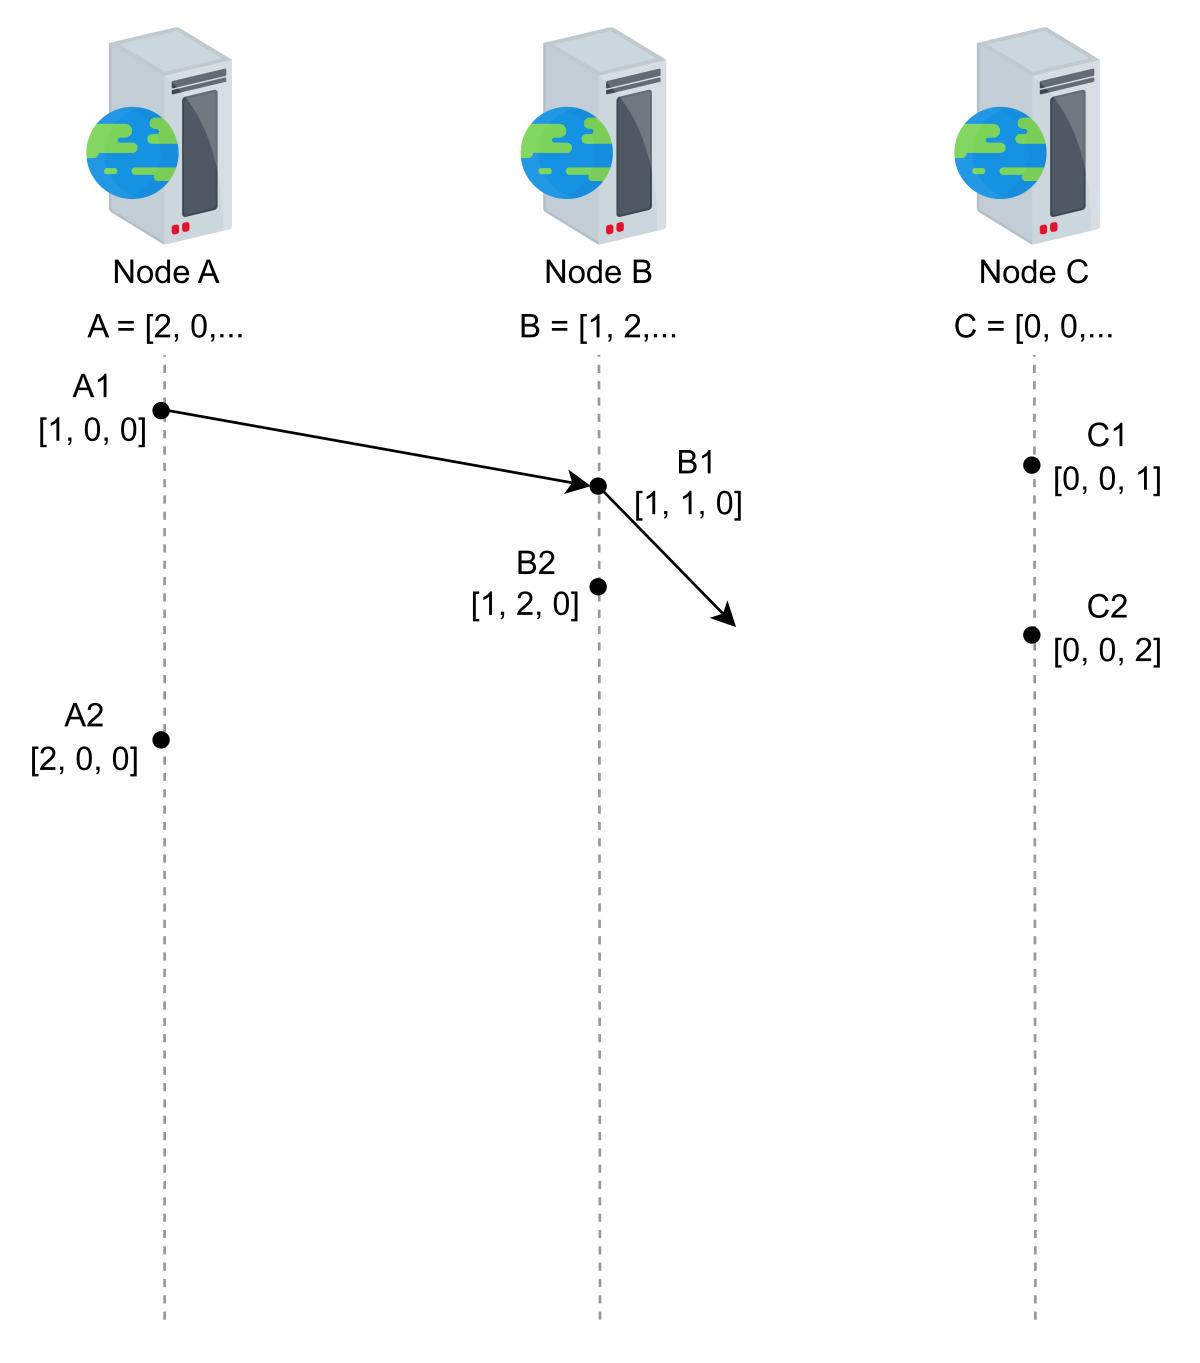
\includegraphics[width=\textwidth]{Images/chapter_12/section_5836711686307840/6749854270095360.png}
 \caption{Unique ID for A2: [2,0,0][A]}
 \end{subfigure}
\end{figure}

\begin{figure}[htbp]
 \centering
 \begin{subfigure}[b]{0.48\textwidth}
 \centering
 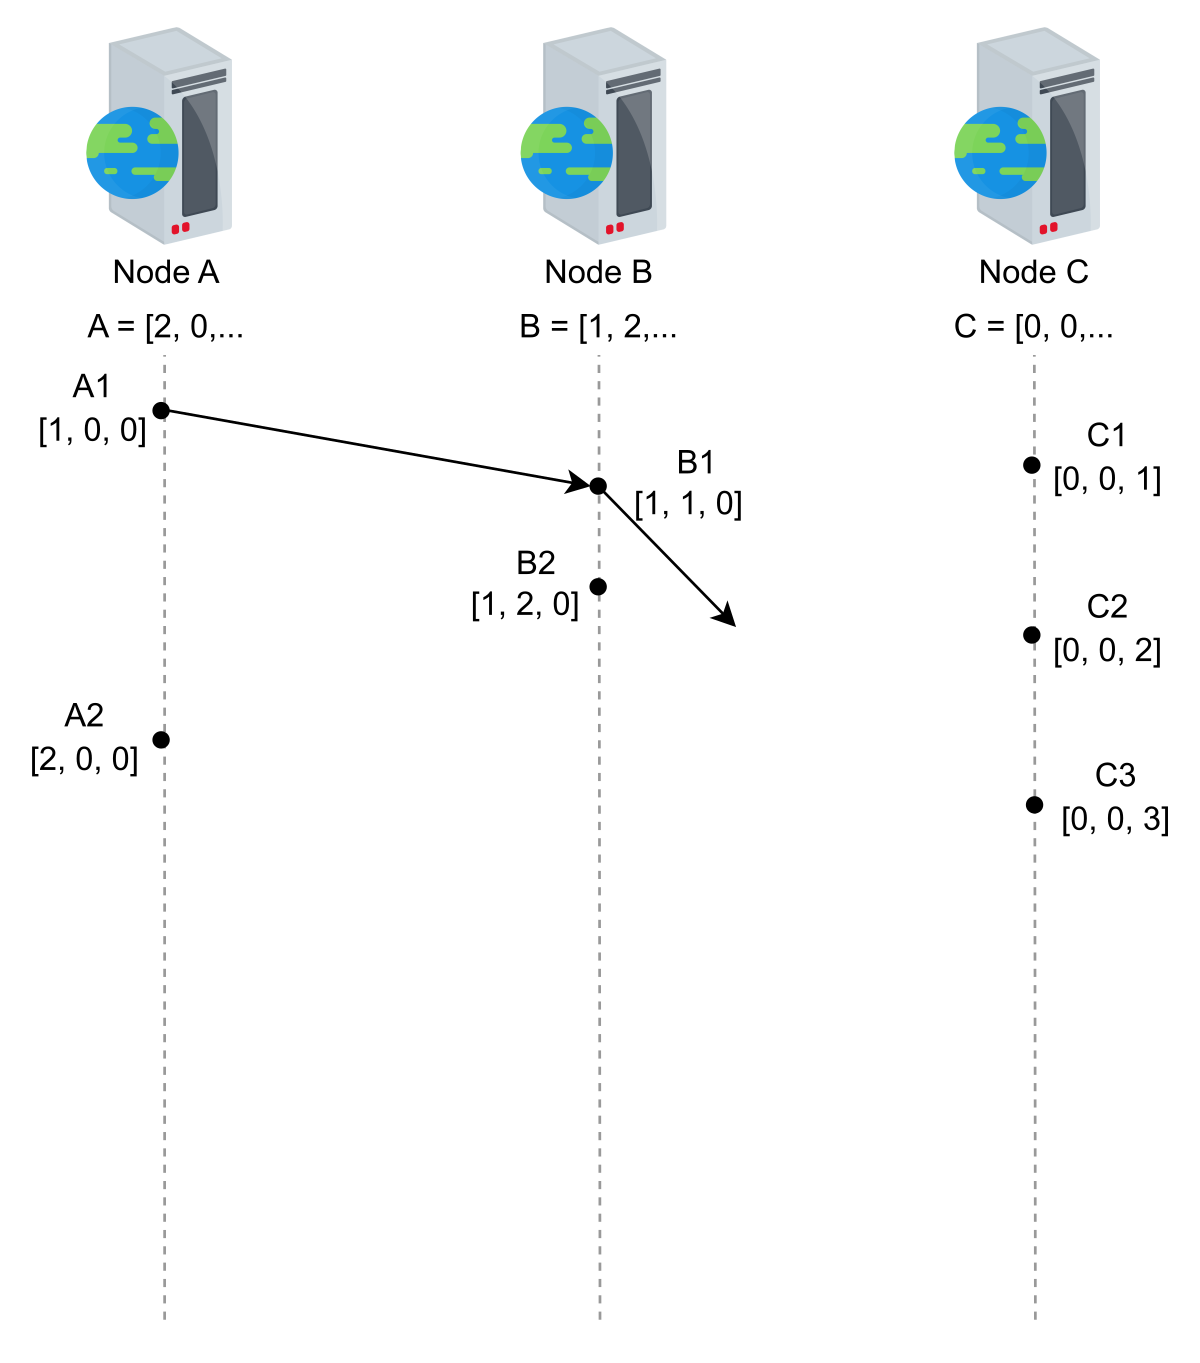
\includegraphics[width=\textwidth]{Images/chapter_12/section_5836711686307840/5612667642183680.png}
 \caption{Unique ID for C3: [0,0,3][C]}
 \end{subfigure}
 \hfill
 \begin{subfigure}[b]{0.48\textwidth}
 \centering
 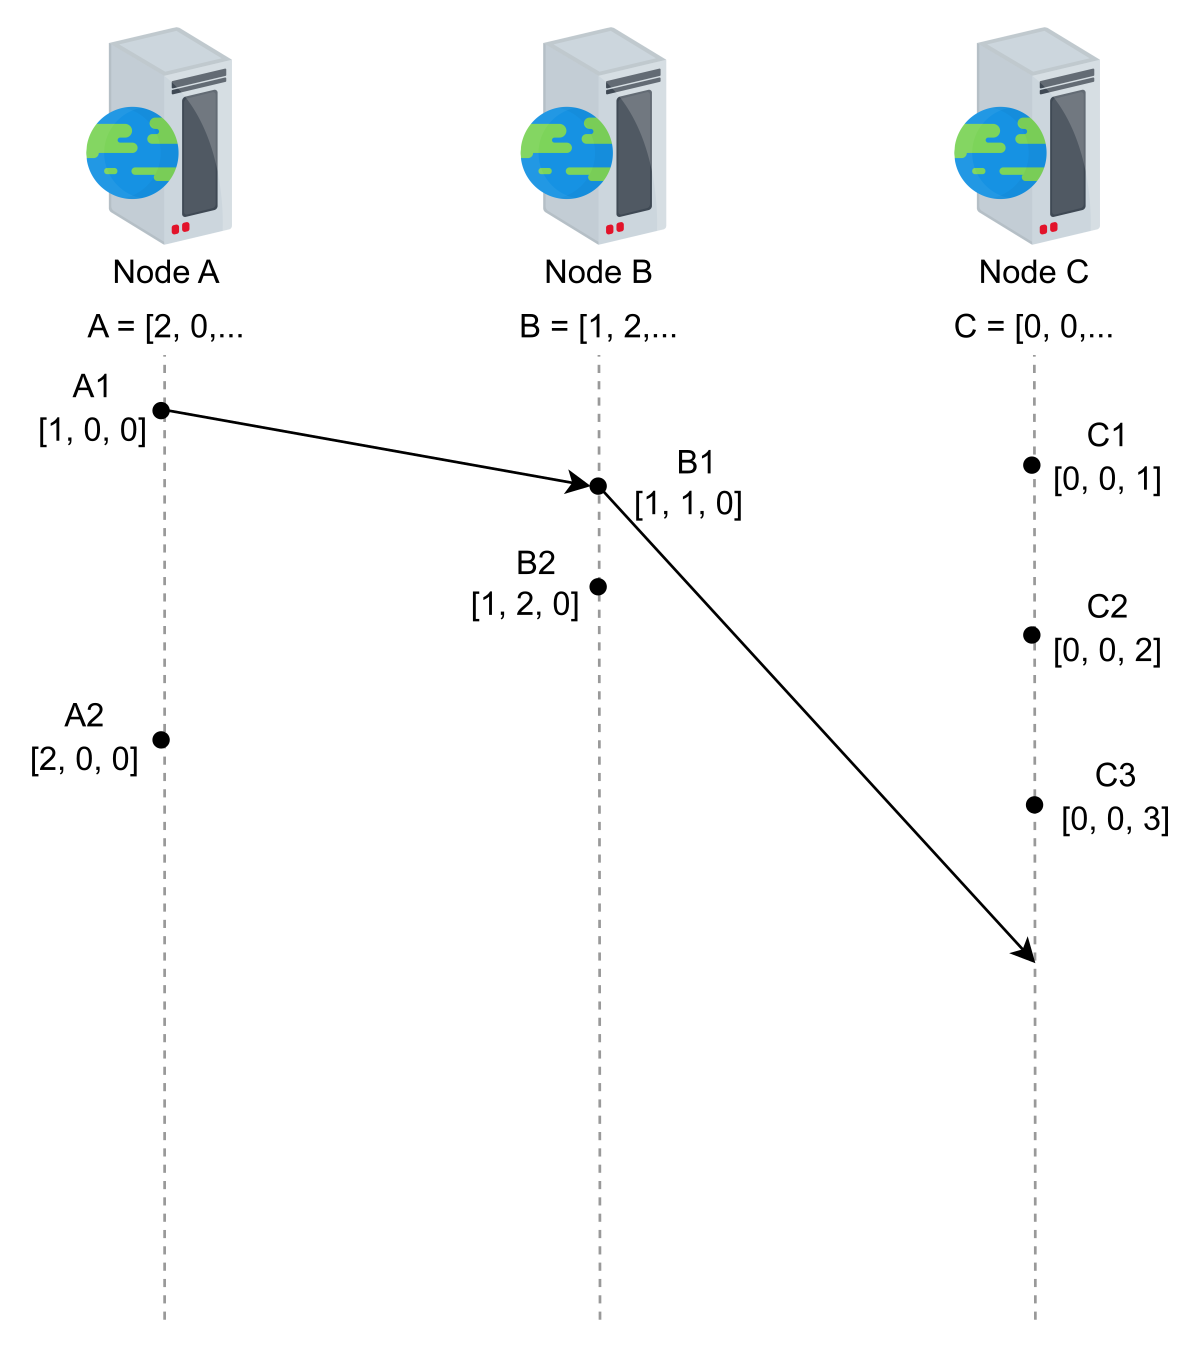
\includegraphics[width=\textwidth]{Images/chapter_12/section_5836711686307840/4555258035306496.png}
 \caption{No new ID needs to be assigned}
 \end{subfigure}
\end{figure}

\begin{figure}[htbp]
 \centering
 \begin{subfigure}[b]{0.48\textwidth}
 \centering
 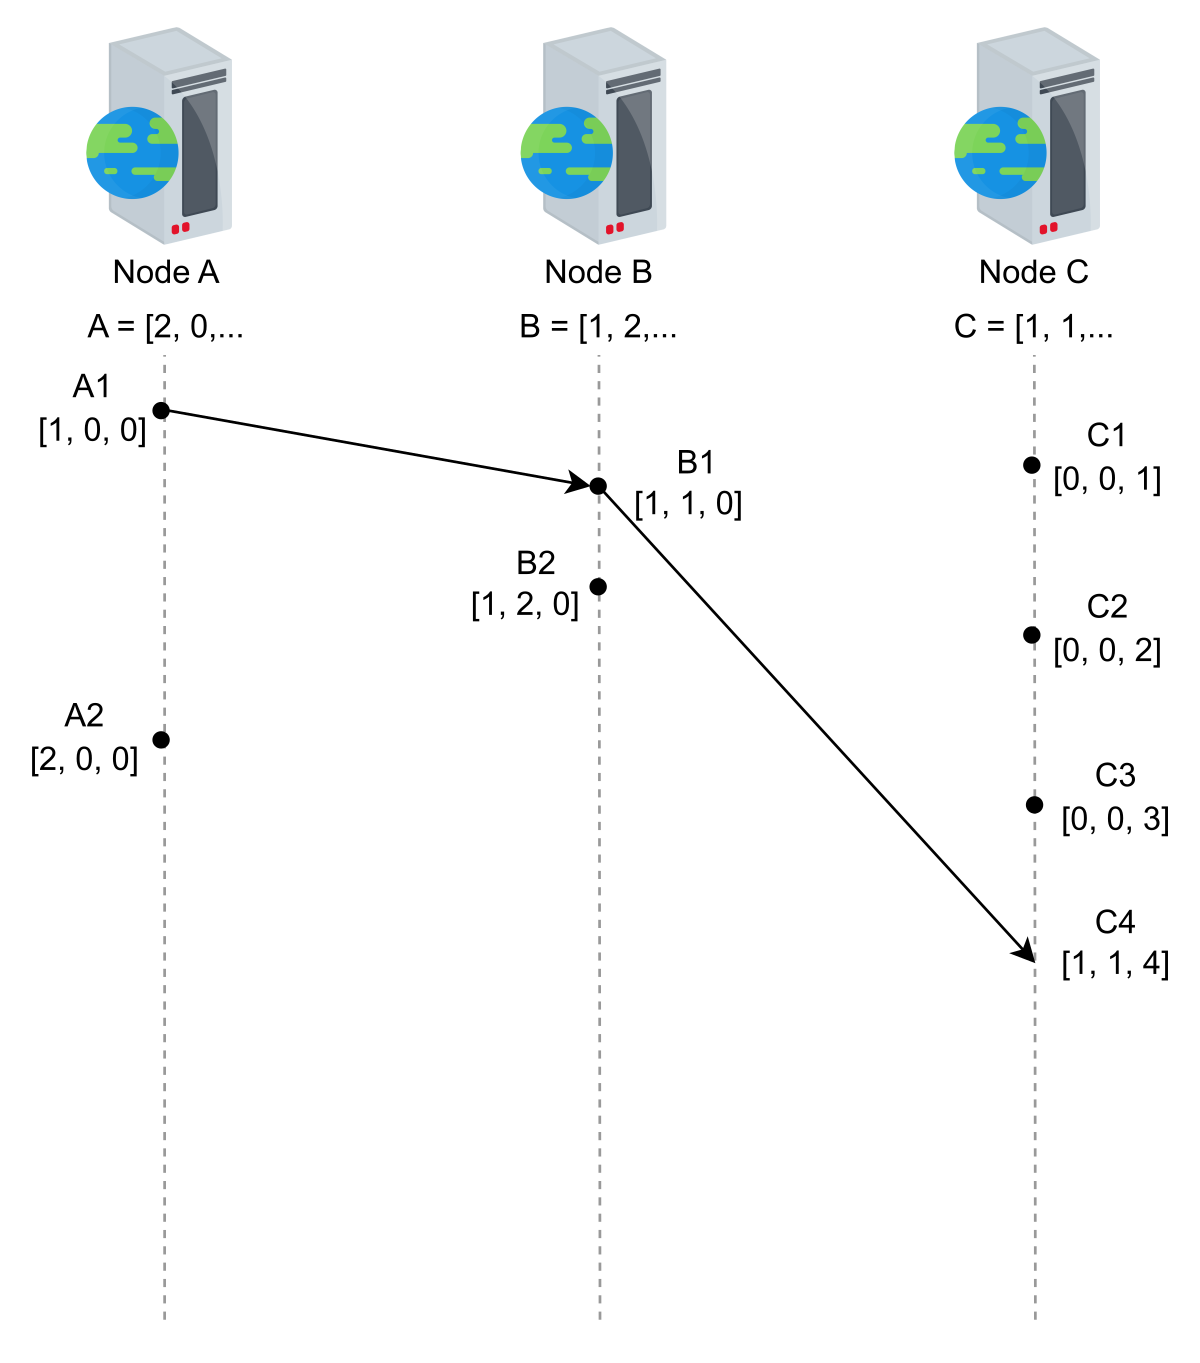
\includegraphics[width=\textwidth]{Images/chapter_12/section_5836711686307840/6681731995140096.png}
 \caption{Unique ID for C4: [1,1,4][C]}
 \end{subfigure}
 \hfill
 \begin{subfigure}[b]{0.48\textwidth}
 \centering
 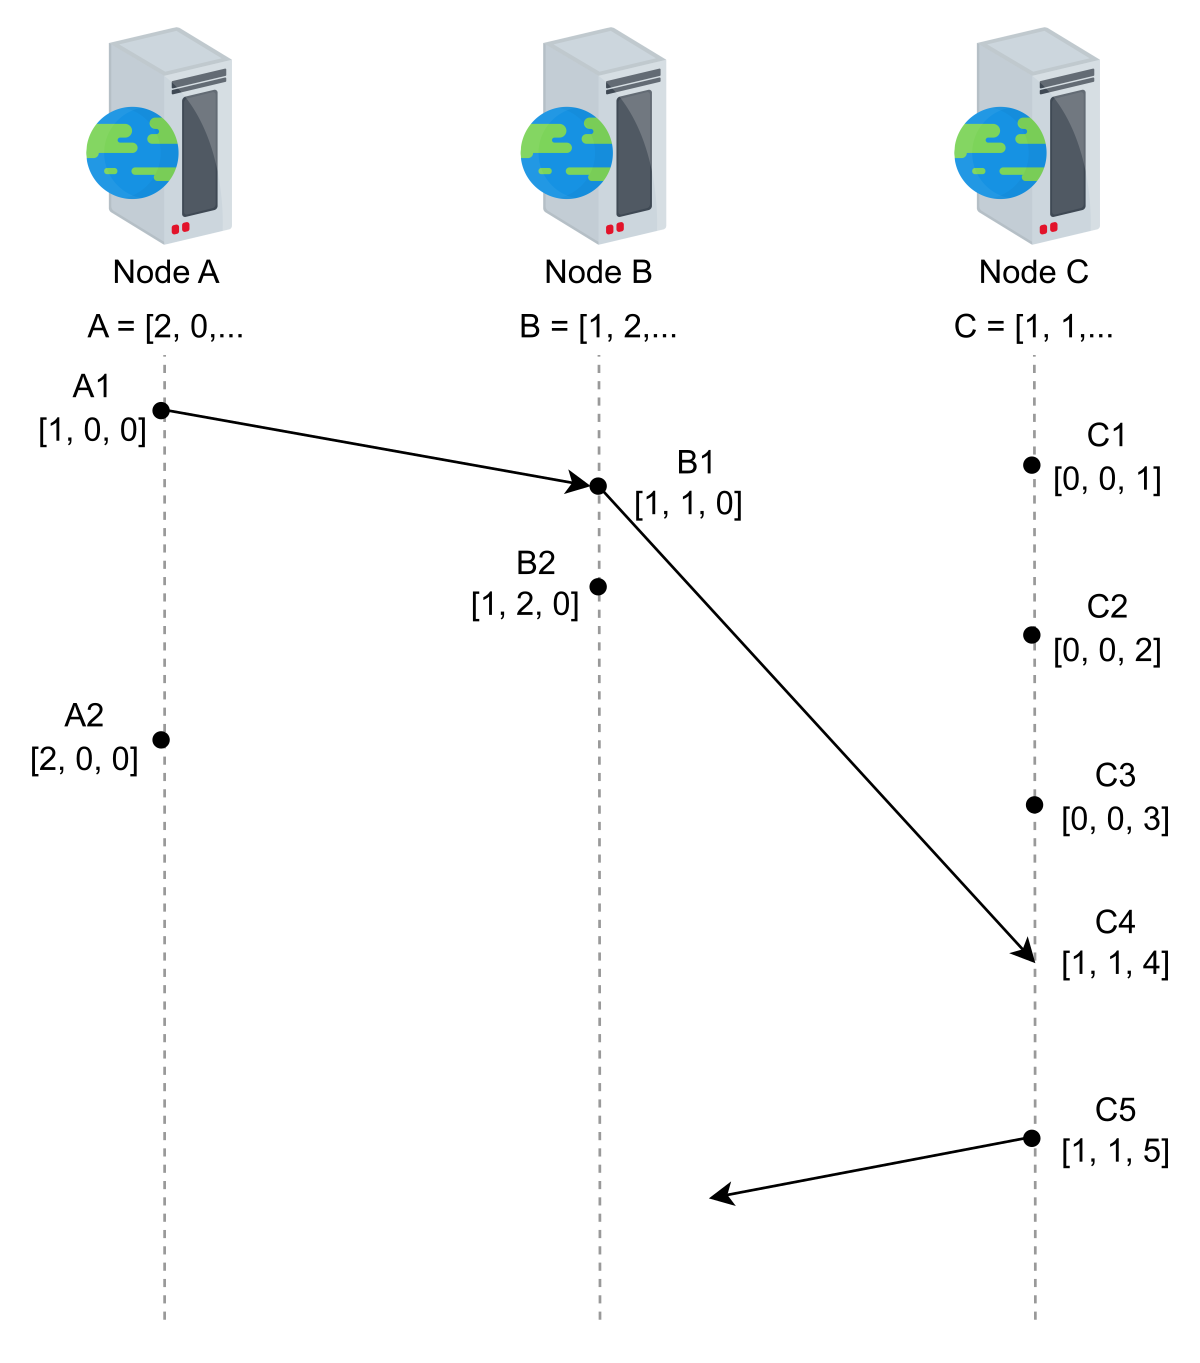
\includegraphics[width=\textwidth]{Images/chapter_12/section_5836711686307840/6631691733827584.png}
 \caption{Unique ID for C5: [1,1,5][C]}
 \end{subfigure}
\end{figure}

\begin{figure}[htbp]
 \centering
 \begin{subfigure}[b]{0.48\textwidth}
 \centering
 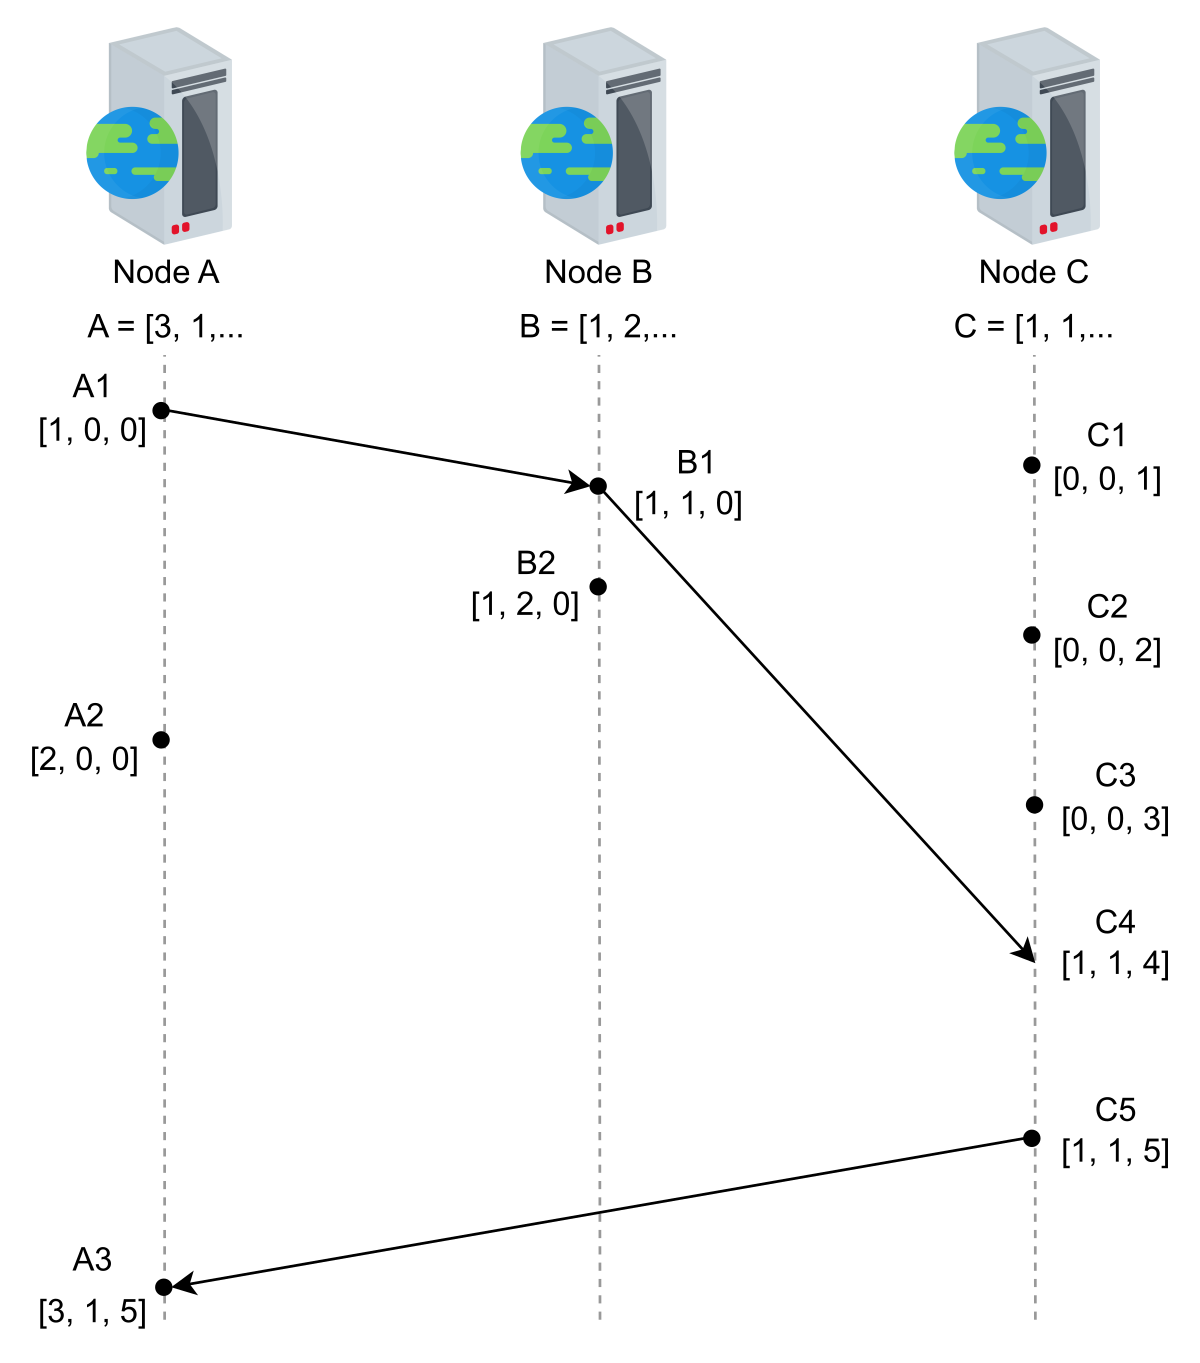
\includegraphics[width=\textwidth]{Images/chapter_12/section_5836711686307840/4847229979197440.png}
 \caption{Unique ID for A3: [3,1,5][A]}
 \end{subfigure}
 \hfill
 \begin{subfigure}[b]{0.48\textwidth}
 \centering
 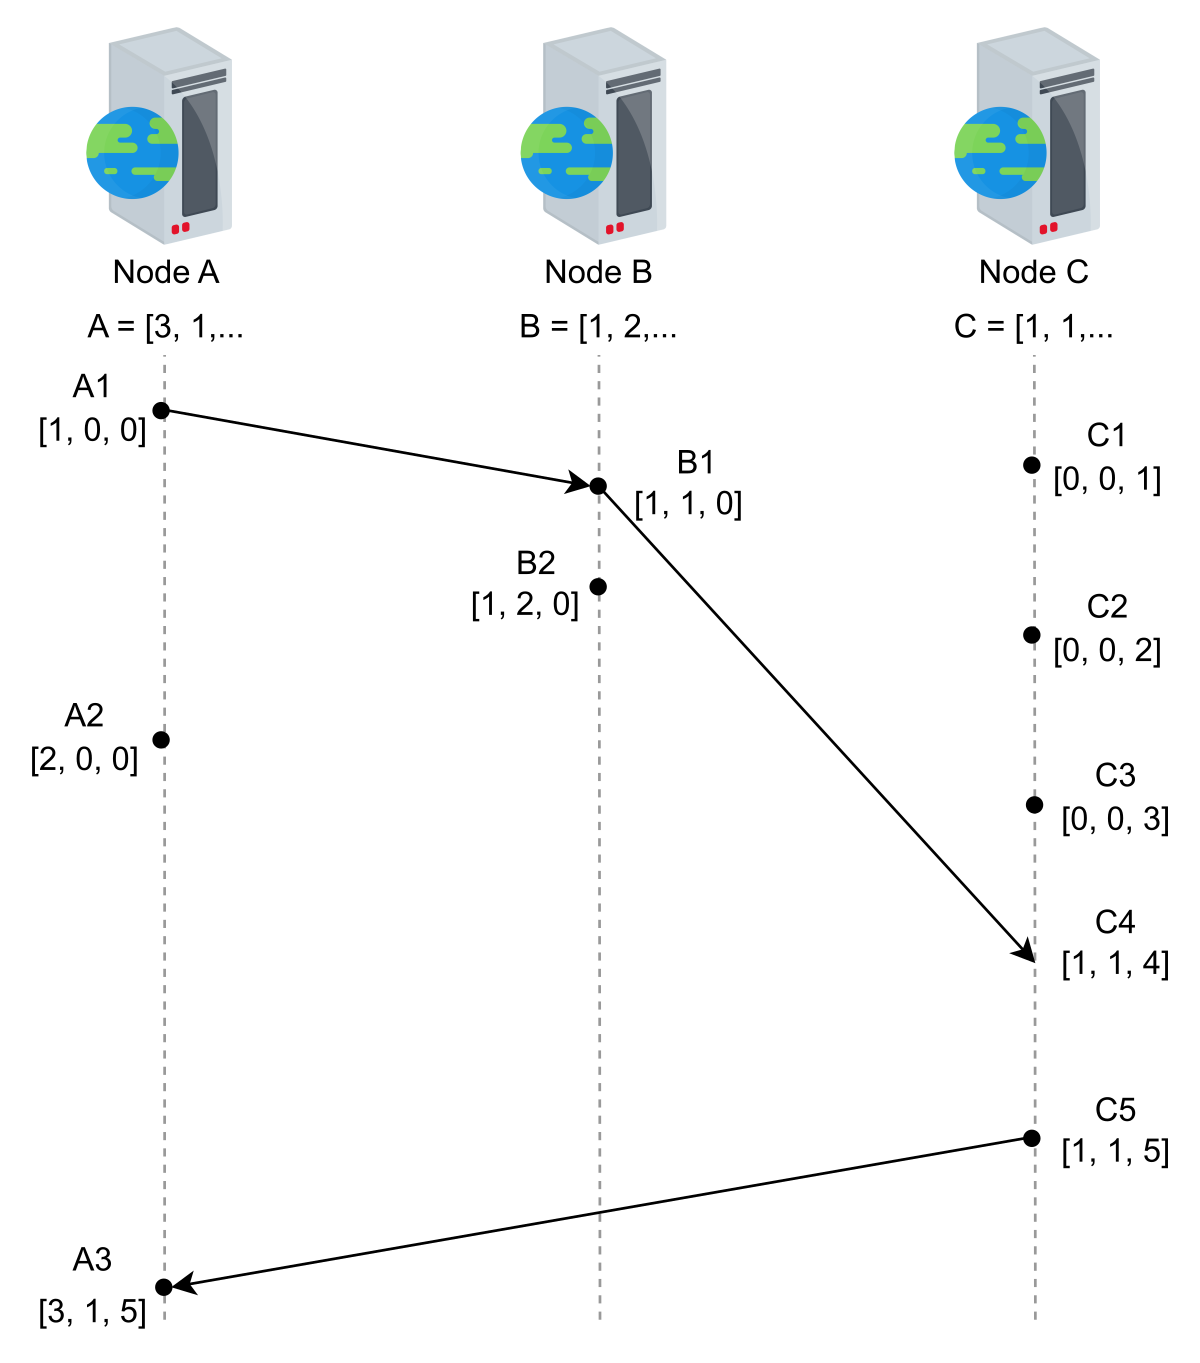
\includegraphics[width=\textwidth]{Images/chapter_12/section_5836711686307840/5200196112613376.png}
 \caption{No new ID needs to be assigned}
 \end{subfigure}
\end{figure}

The slides above explain the vector clock behavior. The system has three nodes, A, B, and C, and the clock tracks events over time at each node. Let 's go through the steps in detail:

\begin{enumerate}
\def\labelenumi{\arabic{enumi}.}
\tightlist
\item
\textbf{Vector clock format (slide 1):} Each node maintains a vector clock {[} A, B, C{]}, where:

\begin{itemize}
\tightlist
\item
A is the local count of events at Node A,
\item
B for Node B, and
\item
C for Node C.
\end{itemize}
\item
\textbf{Event A₁ at Node A (slide 2):}

\begin{itemize}
\tightlist
\item
Clock: {[}1, 0, 0{]}
\item
The first event at node A increments A's clock (the first number in the vector).
\item
Sends a message to B, carrying this clock.
\end{itemize}
\item
\textbf{Events C₁ at Node C (slide 3):}

\begin{itemize}
\tightlist
\item
A local event occurs at node C, which increments C's counter to C₁: {[}0, 0, 1{]}.
\end{itemize}
\item
\textbf{Event B₁ at Node B (slides 4 and 5):}

\begin{itemize}
\item
Node B receives a message generated by node A, with clock A₁: {[}1, 0, 0{]}.
\item
Node B compares the clock with its own {[}0, 0, 0{]}, takes element-wise max, and increments B's counter.
\item
Max is : {[}1, 0, 0{]}, and B increments the clock, which results in B₁: {[}1, 1, 0{]}.
\item
Node B sends a message to node C with a vector clock {[}1, 1, 0{]}.
\end{itemize}
\item
\textbf{Events C₂ at Node C (slide 6):}

\begin{itemize}
\tightlist
\item
A local event occurs at node C, incrementing its vector {[}0, 0, 1{]} to C₂: {[}0, 0, 2{]}.
\end{itemize}
\item
\textbf{Event B₂ at Node B (slide 7):}

\begin{itemize}
\tightlist
\item
A local event occurs at node B, incrementing B's clock from {[}1, 1, 0{]} to {[}1, 2, 0{]}.
\end{itemize}
\item
\textbf{Event A₂ at Node A (slide 8):}

\begin{itemize}
\tightlist
\item
A local event occurs at A, incrementing A's clock to {[}2, 0, 0{]}.
\end{itemize}
\item
\textbf{Events C₃ at Node C (slide 9):}

\begin{itemize}
\tightlist
\item
A local event occurs at node C, incrementing its counter from {[}0, 0, 2{]} to C₃: {[}0, 0, 3{]}.
\end{itemize}
\item
\textbf{Event C₄ at Node C (slides 10 and 11):}

\begin{itemize}
\tightlist
\item
Node C receives a message from B with a vector clock B₂: {[}1, 1, 0{]}.
\item
The current C's clock is {[}0, 0, 3{]}.
\item
C takes max element-wise between {[}0, 0, 3{]} and {[}1, 1, 0{]}, which results in {[}1, 1, 3{]}. The node C then increments its counter; the resultant clock at C is {[}1, 1, 4{]}.
\end{itemize}
\item
\textbf{Event C₅ at Node C (slide 12):}

\begin{itemize}
\tightlist
\item
A local event occurs at node C, incrementing the C's counter to {[}1, 1, 5{]}.
\item
The node C sends a message to A with a vector clock {[}1, 1, 5{]}.
\end{itemize}
\item
\textbf{Event A₃ at Node A (slide 13):}

\begin{itemize}
\tightlist
\item
Node A receives a message from node C with a vector clock {[}1, 1, 5{]}.
\item
Node A's local clock was {[}2, 0, 0{]}.
\item
Node A takes max element-wise between {[}1, 1, 5{]} and {[}2, 0, 0{]}, which results in {[}2, 1, 5{]}.
\item
Node increases its counter, the resultant clock at Node A is {[}3, 1, 5{]}.
\end{itemize}
\item
\textbf{The final vector clock states (slide 14):}

\begin{itemize}
\tightlist
\item
A = {[}3, 1, 5{]}.
\item
B = {[}1, 2, 0{]}.
\item
C = {[}1, 1, 5{]}.
\end{itemize}
\end{enumerate}

Our approach with vector clocks works. However, in order to completely capture causality, a vector clock must be at least \protect\phantomsection\label{katex_inline_3oVYVcul2l_qf_hg5hQKJ}{{{\(n\)}}} nodes in size. As a result, when the total number of participating nodes is enormous, vector clocks require a significant amount of storage. Some systems nowadays, such as web applications, treat every browser as a client of the system. Such information increases the ID length significantly, making it difficult to handle, store, use, and scale.

\textbf{Requirements Fulfilled by Each Approach}

\begin{table}[htbp]
\centering
\small
\adjustbox{max width=\textwidth}{
\begin{tabular}{|p{0.233\textwidth}|p{0.123\textwidth}|p{0.113\textwidth}|p{0.100\textwidth}|p{0.174\textwidth}|p{0.208\textwidth}|}
\hline
\hfill\break & \textbf{Unique} & \textbf{Sca{} lable} & \textbf{Available} & \textbf{64-bit numeric ID} & \textbf{Causality maintained} \\
\hline
\hline
\textbf{Using UUID} & no & yes & yes & no & no \\
\hline
\textbf{Using a database} & no & no & yes & yes & no \\
\hline
\textbf{Using a range handler} & yes & yes & yes & yes & no \\
\hline
\textbf{Using UNIX time stamps} & no & \textbf{weak} & yes & yes & \textbf{weak} \\
\hline
\textbf{Using Twitter Snowflake} & yes & yes & yes & yes & \textbf{weak} \\
\hline
\textbf{Using vector clocks} & yes & \textbf{weak} & yes & \textbf{can exceed} & yes \\
\hline
\end{tabular}
}
\caption{Requirements Fulfilled by Each Approach}
\end{table}

\begin{quote}
\textbf{Quiz:}
\textbf{Question 1:} Would a global clock help solve our problem?
\textbf{Answer:} Since we don't have a global clock, even if each node can assign unique time stamps to the events happening, these time stamps will come from clocks running at different rates. This would make it harder to compare them, and they won't be unique. However, if we have a global clock that gives us time upon request and is always accurate, then we can maintain the causality of events, as well as a unique ID. Such a clock would be significantly valuable, but time is tricky to handle in distributed systems.
\end{quote}

\subsection{TrueTime API}\label{liqtnAoz6gE5qq4rqXycv}
\\
Google's TrueTime API(Spanner: Google's Globally-Distributed Database, Google, Inc.) in Spanner is an interesting option. Instead of a particular time stamp, it reports an interval of time. When asking for the current time, we get back two values: the earliest and latest ones. These are the earliest possible and latest possible time stamps.
\\
Based on its uncertainty calculations, the clock knows that the actual current time is somewhere within that interval. The width of the interval depends, among other things, on how long it has been since the local quartz clock was last synchronized with a more accurate clock source.
\\
Google deploys a GPS receiver or atomic clock in each data center, and clocks are synchronized within about 7 ms. This allows Spanner to keep the clock uncertainty to a minimum. The uncertainty of the interval is represented as epsilon.
\\
The following slides explain how TrueTime's time master servers work with GPS and atomic clocks in multiple data centers.

\begin{figure}[htbp]
 \centering
 \begin{subfigure}[b]{0.48\textwidth}
 \centering
 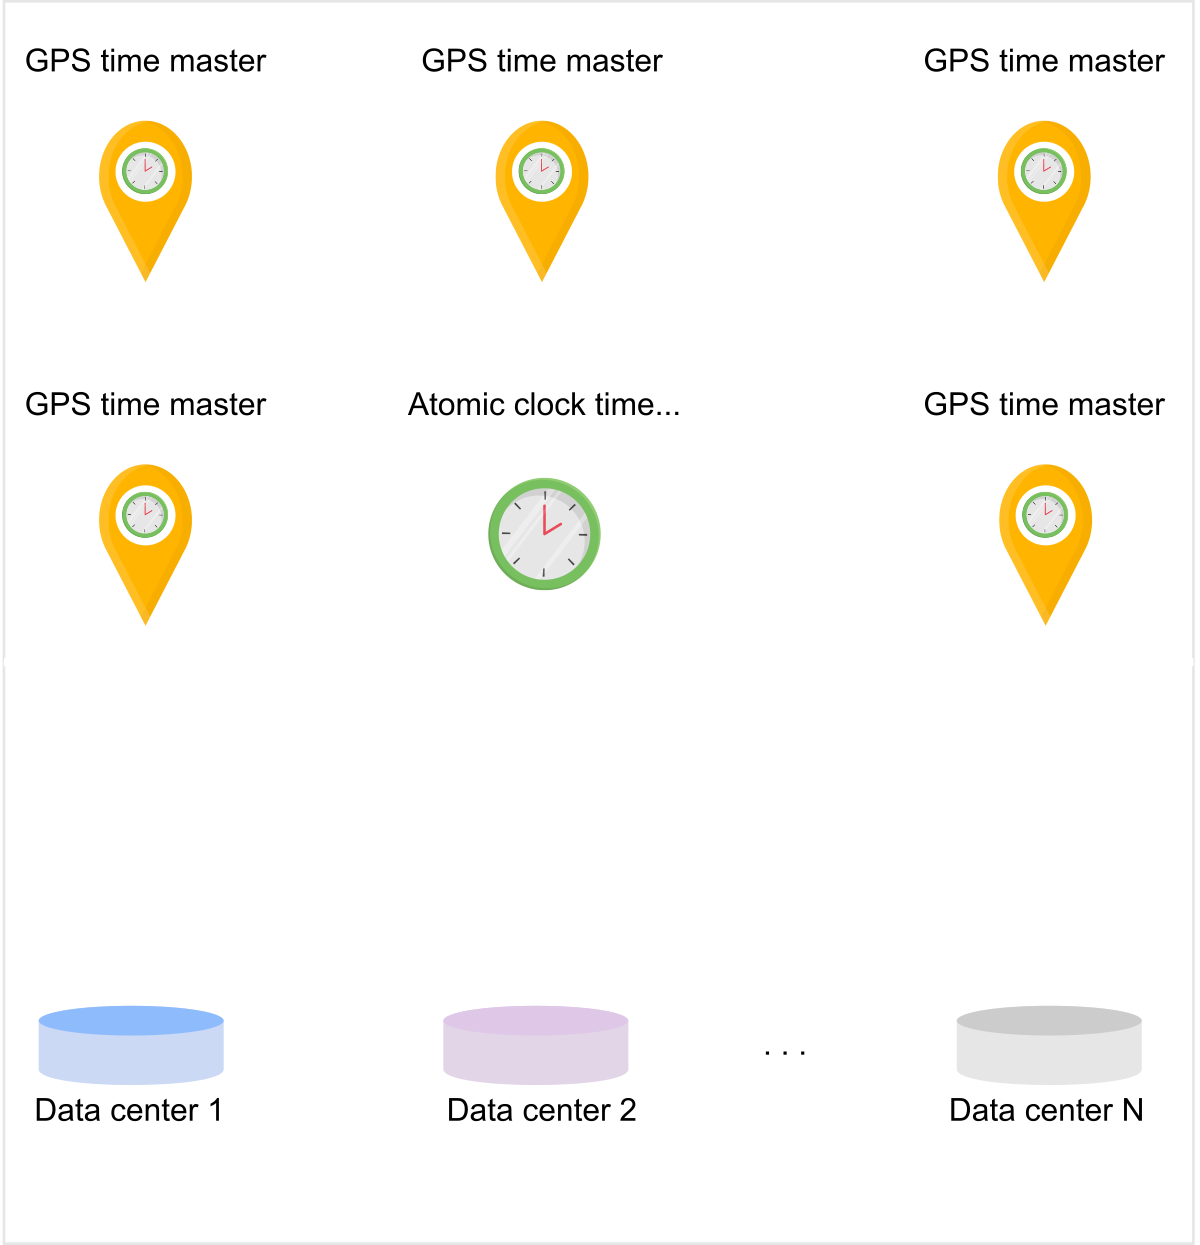
\includegraphics[width=\textwidth]{Images/chapter_12/section_5836711686307840/5613601314439168.png}
 \caption{In every data center, we have time handlers. GPS timemasters have GPS receivers attached, and few of them have atomic clocks}
 \end{subfigure}
 \hfill
 \begin{subfigure}[b]{0.48\textwidth}
 \centering
 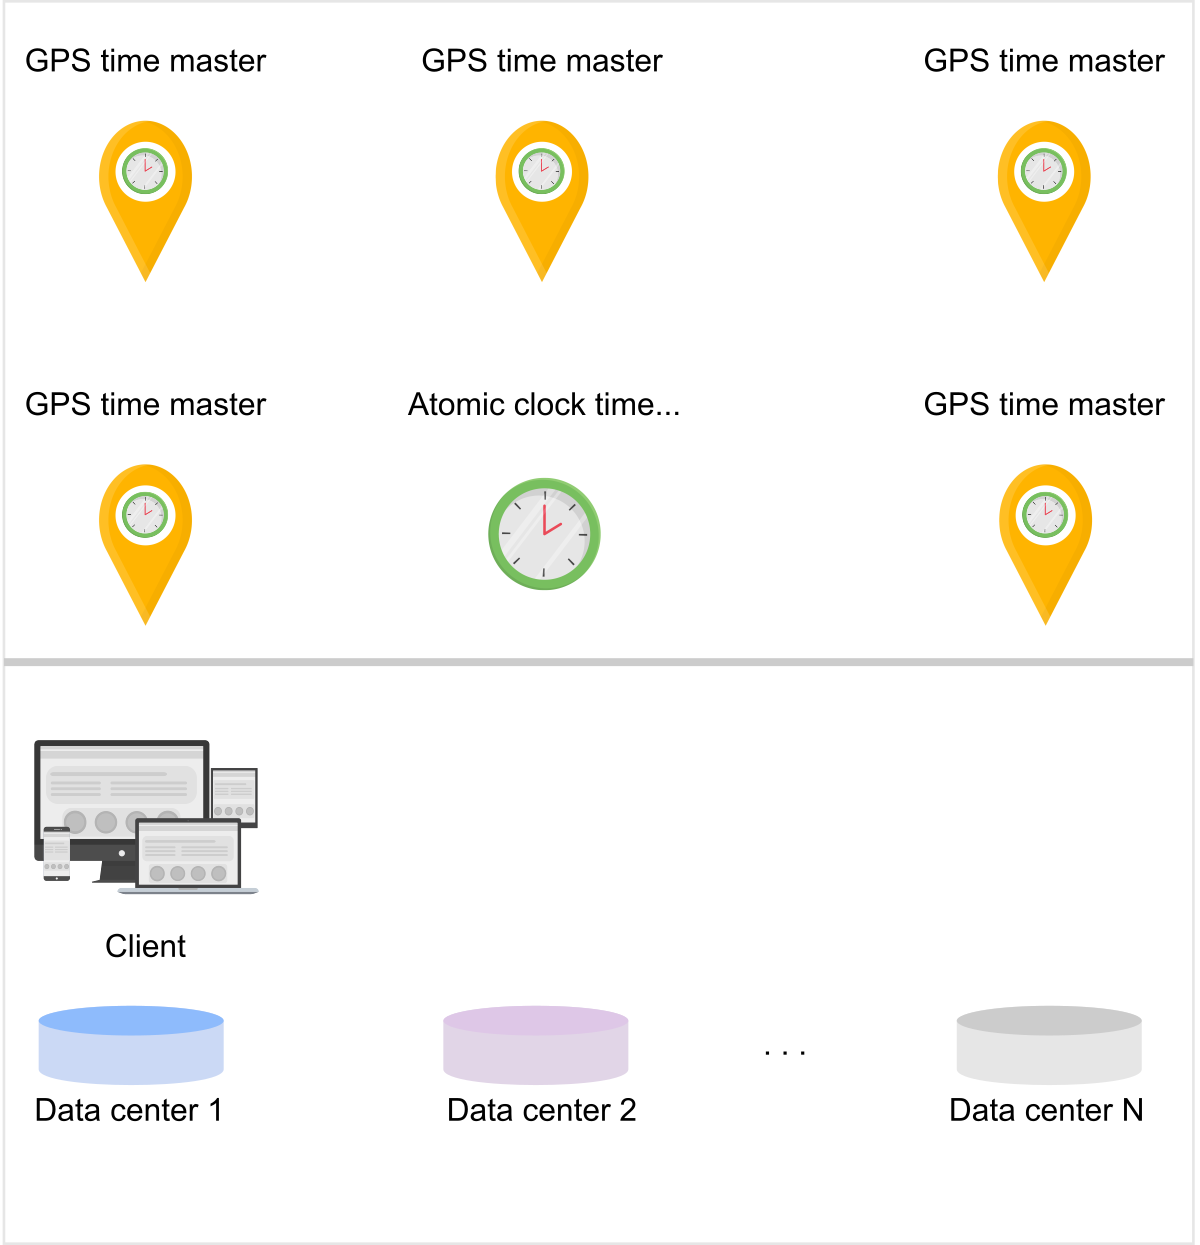
\includegraphics[width=\textwidth]{Images/chapter_12/section_5836711686307840/5300123999535104.png}
 \caption{A client needs a TrueTime}
 \end{subfigure}
\end{figure}

\begin{figure}[htbp]
 \centering
 \begin{subfigure}[b]{0.48\textwidth}
 \centering
 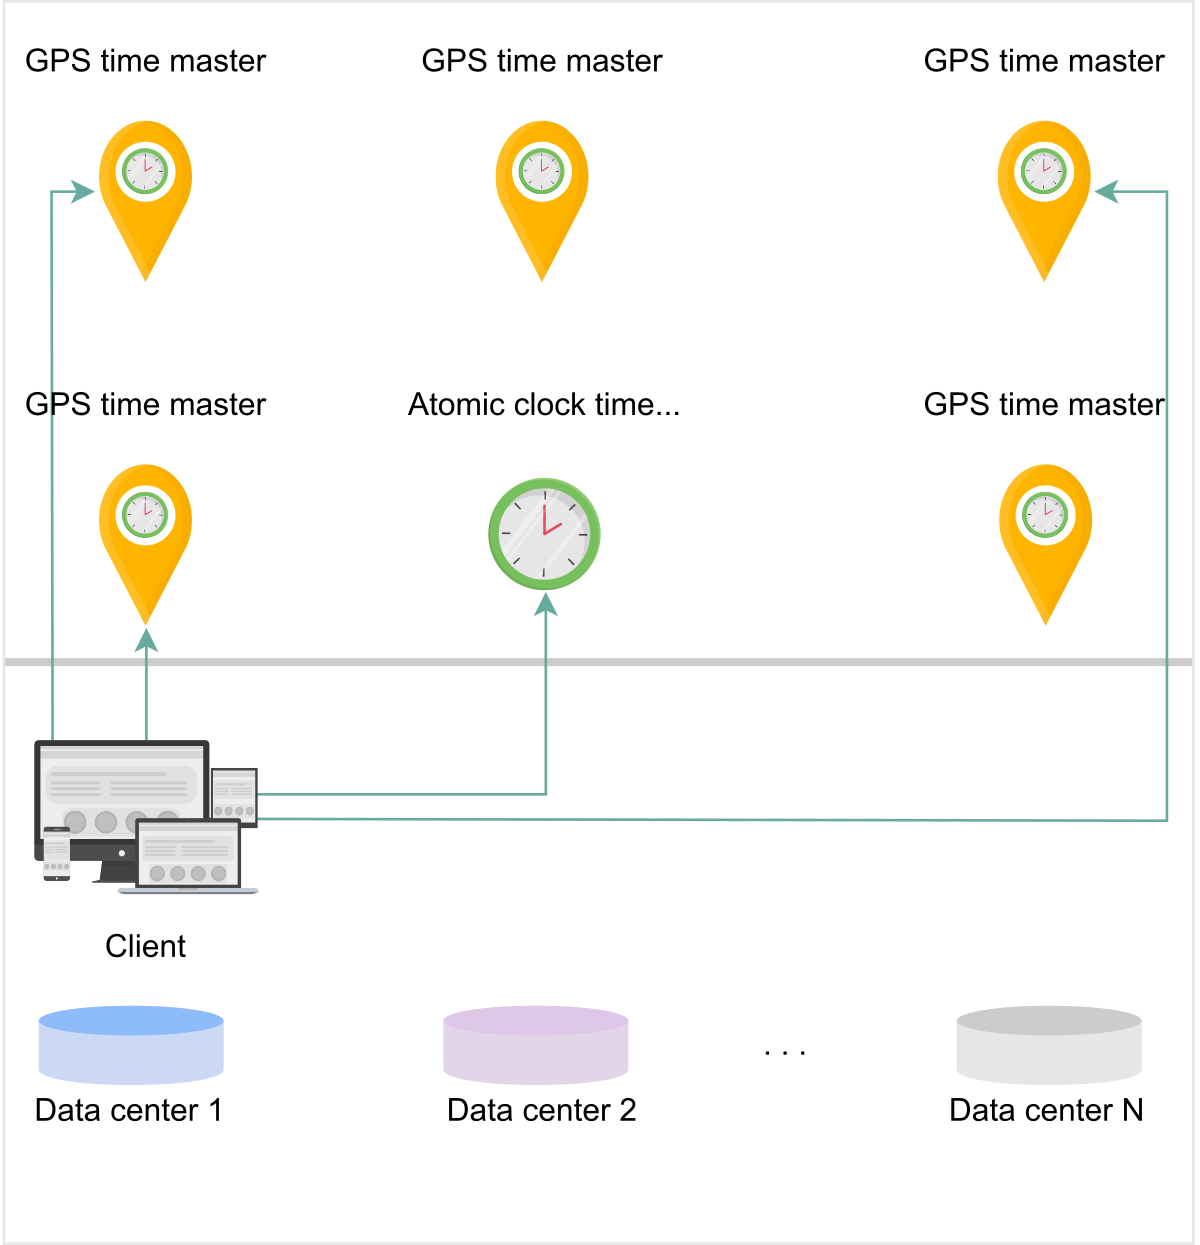
\includegraphics[width=\textwidth]{Images/chapter_12/section_5836711686307840/4770832832397312.png}
 \caption{A client runs a daemon. The daemon contacts mostly GPS time masters and sometimes will contact atomic clock time masters to get the redundancy of different time references}
 \end{subfigure}
 \hfill
 \begin{subfigure}[b]{0.48\textwidth}
 \centering
 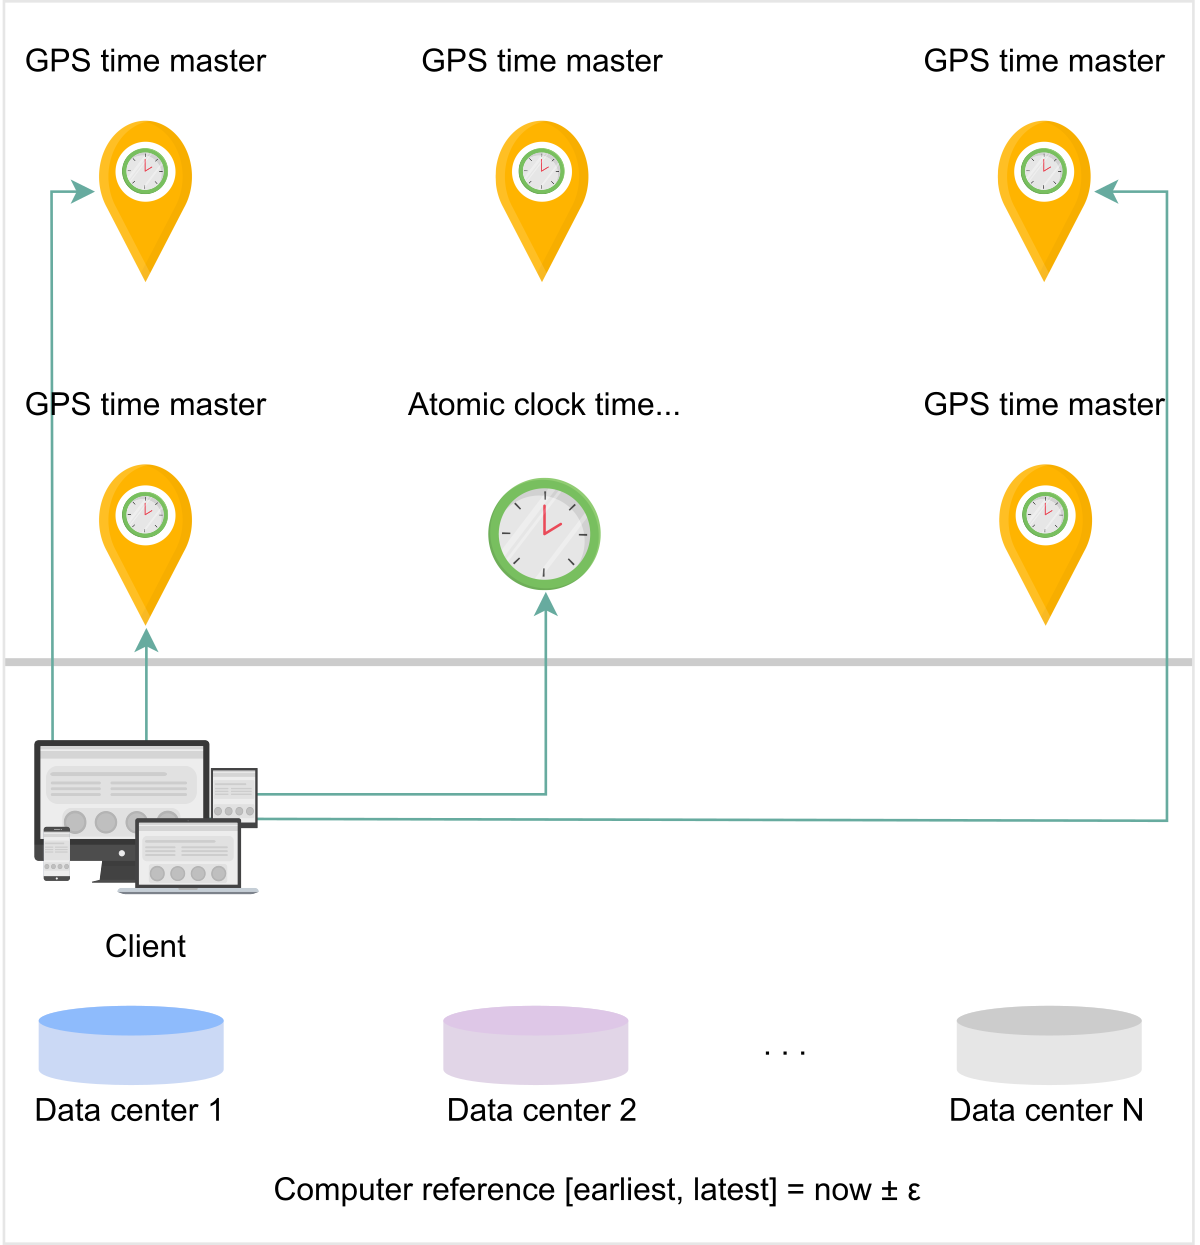
\includegraphics[width=\textwidth]{Images/chapter_12/section_5836711686307840/5175928124735488.png}
 \caption{We run Marzullo's algorithm, which intersects time intervals to determine a time reference. The API gives an interval from earliest to latest}
 \end{subfigure}
\end{figure}

\begin{figure}[htbp]
 \centering
 \begin{subfigure}[b]{0.48\textwidth}
 \centering
 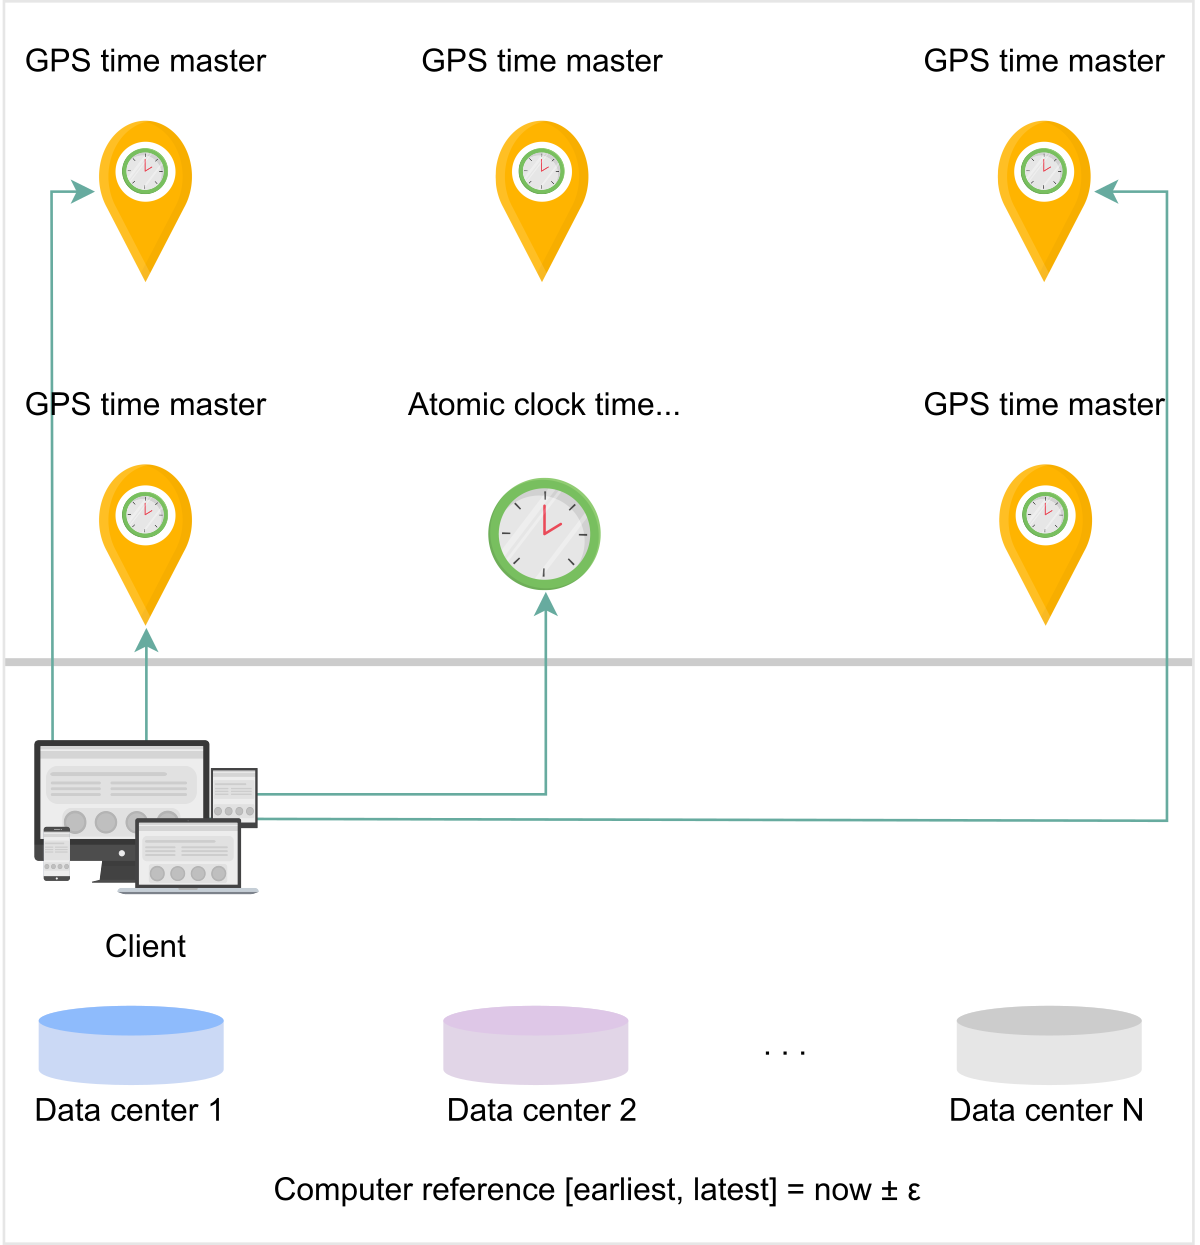
\includegraphics[width=\textwidth]{Images/chapter_12/section_5836711686307840/4803628397363200.png}
 \caption{The time reference will express a given interval as plus or minus epsilon}
 \end{subfigure}
\end{figure}

The following slides explain how time is calculated when the client asks to give TrueTime.

\begin{figure}[htbp]
 \centering
 \begin{subfigure}[b]{0.48\textwidth}
 \centering
 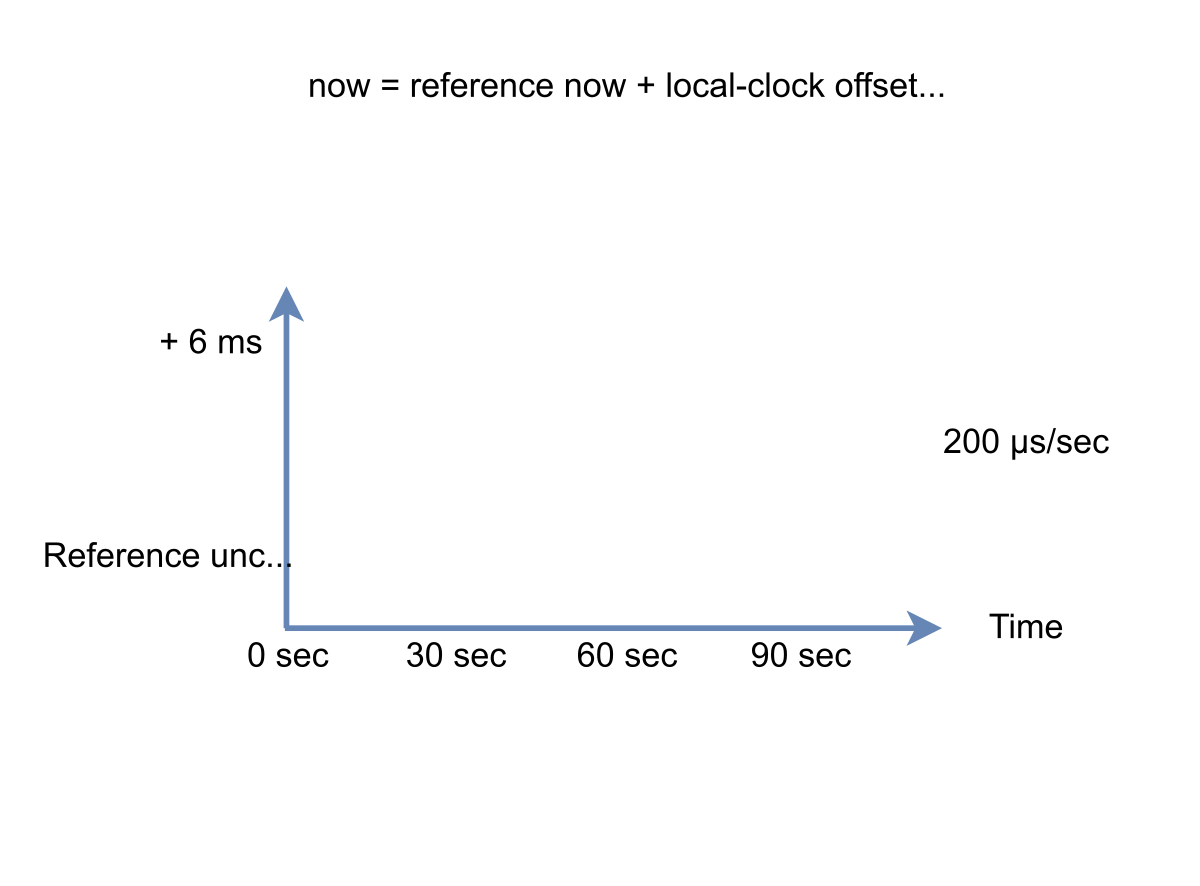
\includegraphics[width=\textwidth]{Images/chapter_12/section_5836711686307840/4870733465649152.png}
 \caption{Before the client asks for TrueTime}
 \end{subfigure}
 \hfill
 \begin{subfigure}[b]{0.48\textwidth}
 \centering
 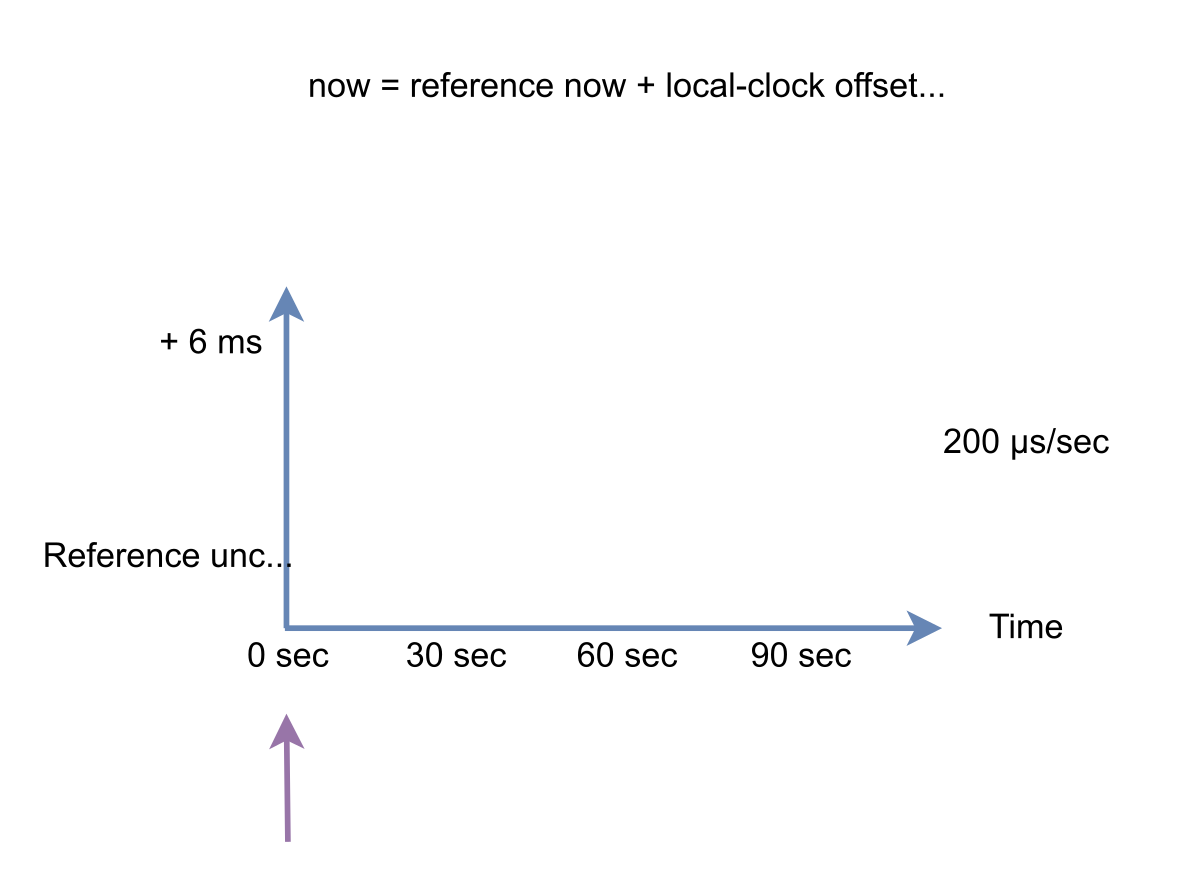
\includegraphics[width=\textwidth]{Images/chapter_12/section_5836711686307840/6589833367781376.png}
 \caption{Compute epsilon at time zero}
 \end{subfigure}
\end{figure}

\begin{figure}[htbp]
 \centering
 \begin{subfigure}[b]{0.48\textwidth}
 \centering
 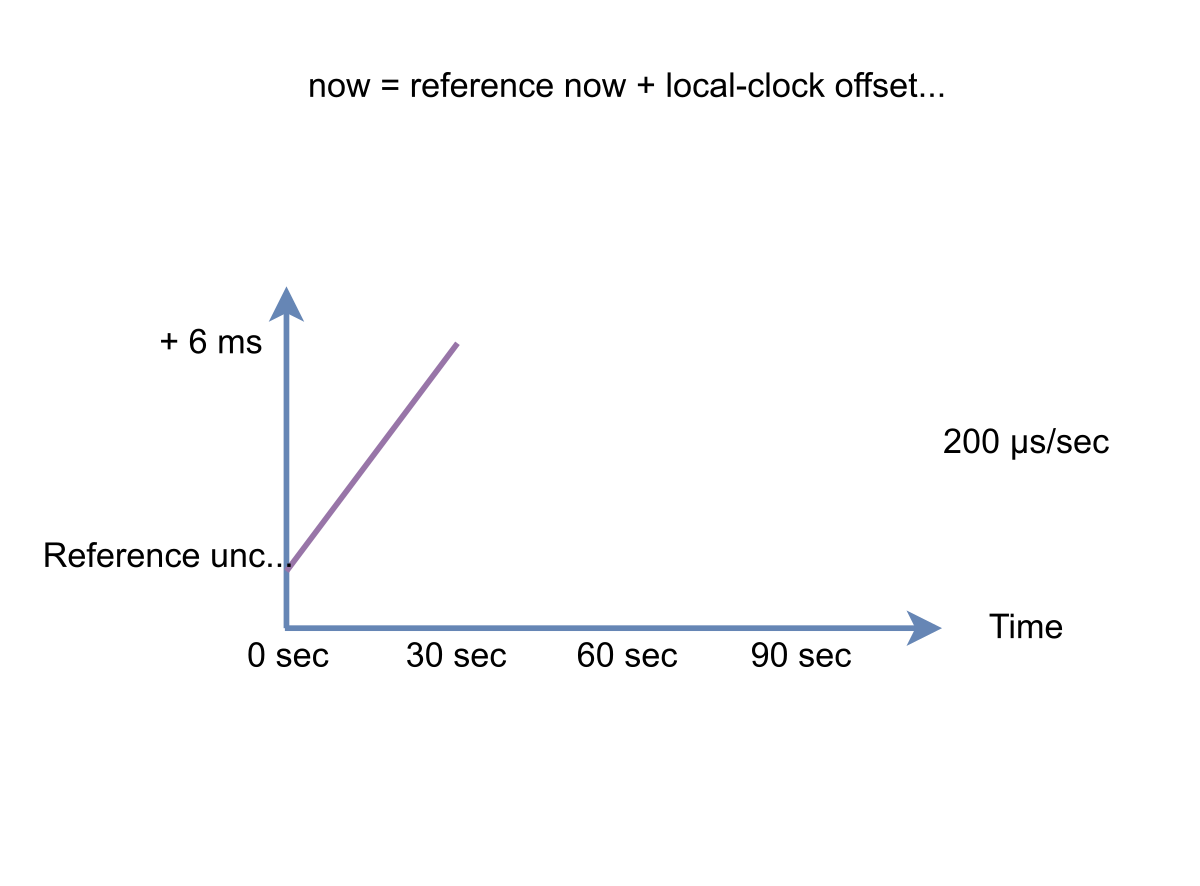
\includegraphics[width=\textwidth]{Images/chapter_12/section_5836711686307840/6077527588339712.png}
 \caption{We’ll assume that the clock drifts at most, 200 microseconds per second. This means we’ll roughly add 6 milliseconds (ms) on to the value of epsilon over 30 seconds}
 \end{subfigure}
 \hfill
 \begin{subfigure}[b]{0.48\textwidth}
 \centering
 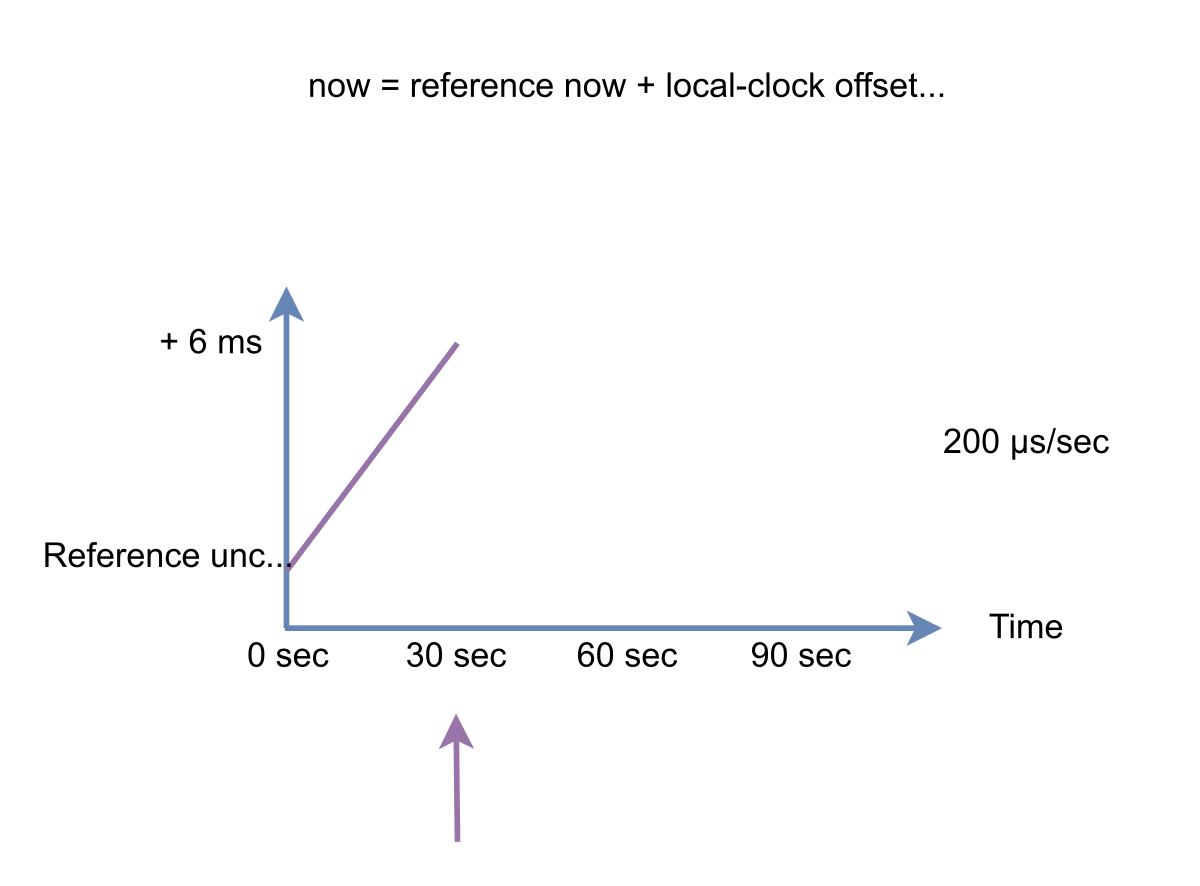
\includegraphics[width=\textwidth]{Images/chapter_12/section_5836711686307840/4585659776106496.png}
 \caption{Compute epsilon at 30 seconds}
 \end{subfigure}
\end{figure}

\begin{figure}[htbp]
 \centering
 \begin{subfigure}[b]{0.48\textwidth}
 \centering
 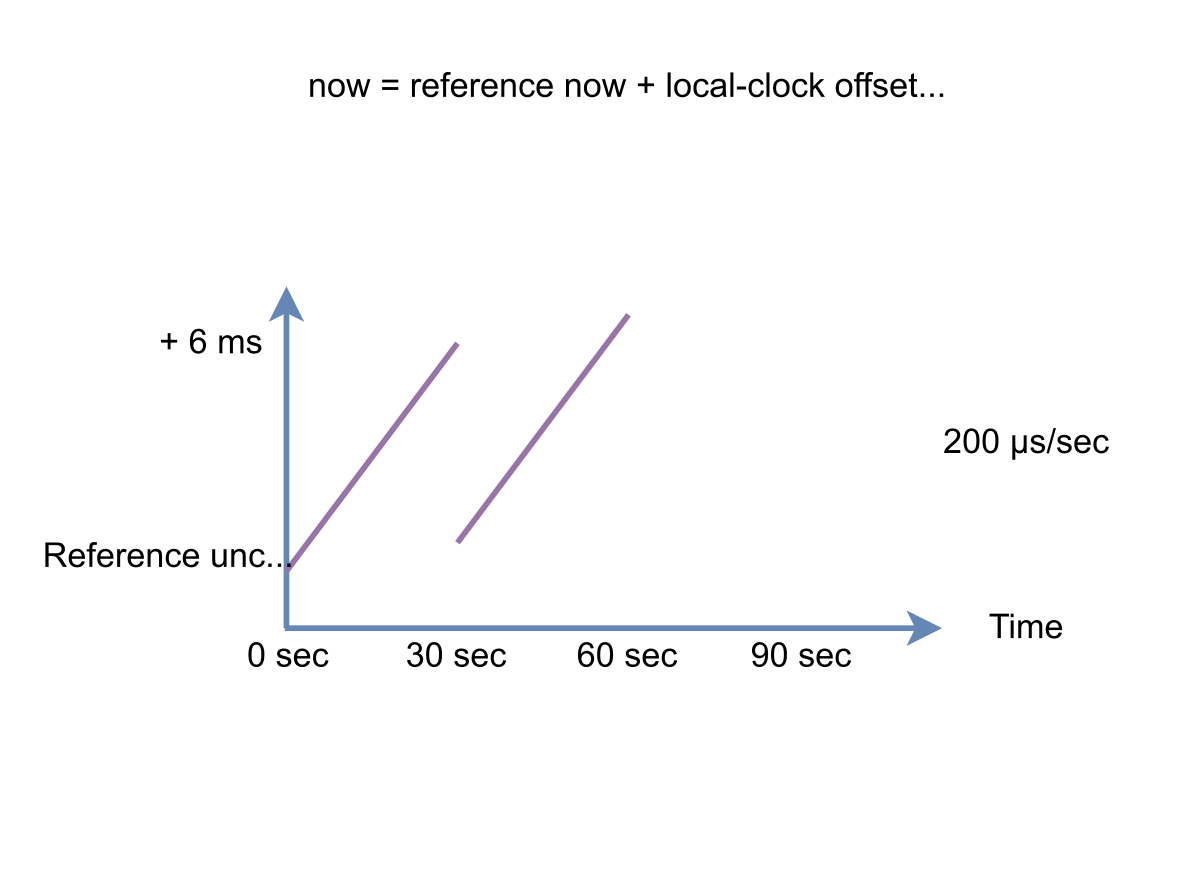
\includegraphics[width=\textwidth]{Images/chapter_12/section_5836711686307840/5625731656974336.png}
 \caption{In the next 30 seconds, we communicate to the time master as reference uncertainty is computed, and it increases at the rate of 200 microseconds per second}
 \end{subfigure}
 \hfill
 \begin{subfigure}[b]{0.48\textwidth}
 \centering
 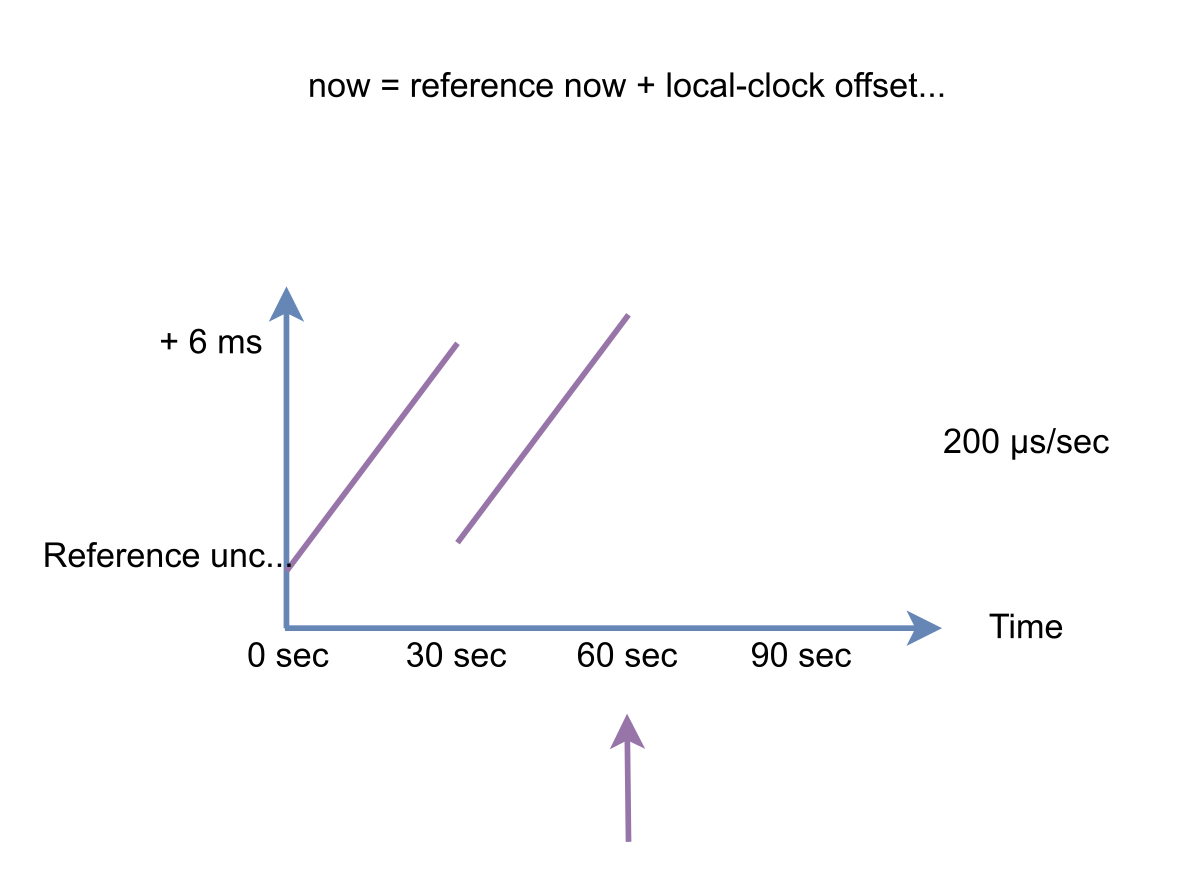
\includegraphics[width=\textwidth]{Images/chapter_12/section_5836711686307840/5362493379837952.png}
 \caption{Compute epsilon at 60 seconds}
 \end{subfigure}
\end{figure}

\begin{figure}[htbp]
 \centering
 \begin{subfigure}[b]{0.48\textwidth}
 \centering
 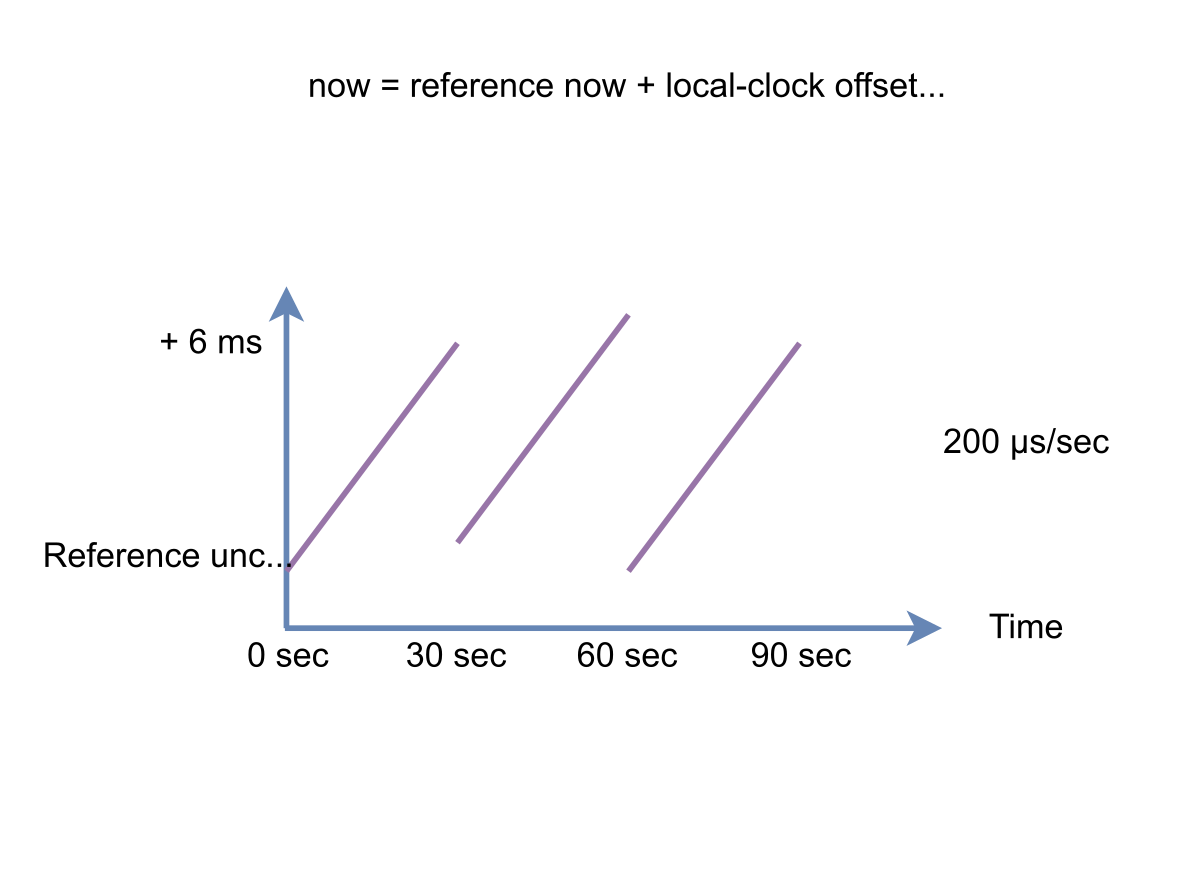
\includegraphics[width=\textwidth]{Images/chapter_12/section_5836711686307840/6167498026385408.png}
 \caption{Again, the computed reference uncertainty increases at the rate of 200 microseconds per second}
 \end{subfigure}
\end{figure}

Spanner guarantees that two confidence intervals don't overlap (that is, \protect\phantomsection\label{katex_inline_833cE8WvDKcLLUCcYhdoI}{{{\(\text{A}_\text{{earliest}}\)}}} \textless{} \protect\phantomsection\label{katex_inline_v5DTpMfepWNGie0yWIe1Z}{{{\(\text{A}_\text{{latest}}\)}}}\textless{} \protect\phantomsection\label{katex_inline_h9A_hJvRKFA6vSbNYBOn5}{{{\(\text{B}_\text{{earliest}}\)}}} \textless{} \protect\phantomsection\label{katex_inline_Y8z_hGm50DN_xA3i6boyJ}{{{\(\text{B}_\text{{latest}}\)}}}), then B definitely happened after A.
\\
We generate our unique ID using TrueTime intervals. Let 's say the earliest interval is \protect\phantomsection\label{katex_inline_Ok-X-meNe7qY9oi8_jdd2}{{{\(\text{T}_\text{{E​}}\)}}}, the latest is \protect\phantomsection\label{katex_inline_y9IS657olcQao8JxyyrS9}{{{\(\text{T}_\text{{L}}\)}}}, and the uncertainty is \texttt{ε}. We use \protect\phantomsection\label{katex_inline_6oF-XeKhqQAPOyxHh355r}{{{\(\text{T}_\text{{E​}}\)}}} \hspace{0pt} in milliseconds as a time stamp in our unique ID.

\begin{itemize}
\item
\protect\phantomsection\label{nAmqdvOJoQAnLBY-Vh_nR}
\textbf{Time stamp}: The time stamp is 41 bits. We use \protect\phantomsection\label{katex_inline_Uz85JomBG6yxxskmlunOY}{{{\(\text{T}_\text{{E​}}\)}}} as a time stamp.
\item
\protect\phantomsection\label{q6a8bCcUS38X4NtWC9CVt}
\textbf{Uncertainty}: The uncertainty is four bits. Since the maximum uncertainty is claimed to be 6--10 ms, we'll use four bits for storing it.
\item
\protect\phantomsection\label{QwOQ-ZSg65CCKHdqGA6zv}
\textbf{Worker number}: This is 10 bits. It gives us \protect\phantomsection\label{katex_inline_Do-L2cyc4xHsKjHFXqnjv}{{{\(2^{10}\)}}} = 1,024 worker IDs.
\item
\protect\phantomsection\label{IjDgcOsaeB2IoigG7G3ra}
\textbf{Sequence number}: This is eight bits. For every ID generated on the server, the sequence number is incremented by one. It gives us \protect\phantomsection\label{katex_inline_FsNmJtmoCaDsitTklOA9d}{{{\(2^{8}\)}}} = 256 combinations. We'll reset it to zero when it reaches 256.
\end{itemize}

\begin{figure}[htbp]
 \centering
 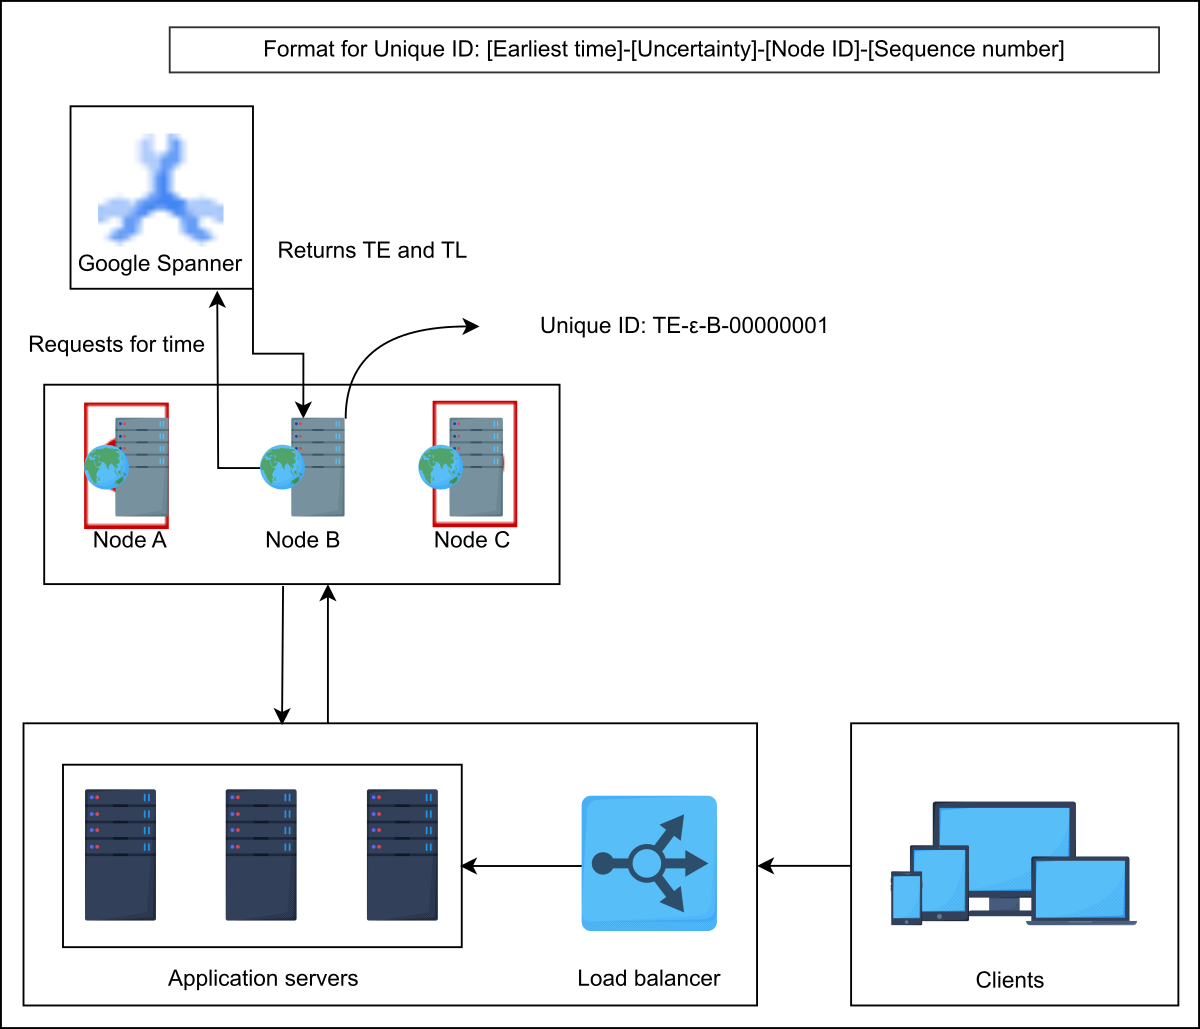
\includegraphics[width=0.5\textwidth]{Images/chapter_12/section_5836711686307840/5890029635633152.png}
 \caption{Node B generating a unique ID for its event using TrueTime}
\end{figure}

\subsubsection{Pros}\label{1ZUOz7bv1gVblWQ8Zr0en}
\\
TrueTime satisfies all the requirements. We're able to generate a globally unique 64-bit identifier. The causality of events is maintained. The approach is scalable and highly available.

\subsubsection{Cons}\label{c9QJgYwwQ3emwdAw9iO61}
\\
If two intervals overlap, then we're unsure in what order A and B occurred. It 's possible that they're concurrent events, but a 100\% guarantee can't be given. Additionally
, Spanner is expensive because it ensures high database consistency. The dollar cost of a Spanner-like system is also high due to its elaborate infrastructure needs and monitoring.
\\
The updated table provides the comparison between the different system designs for generating a unique ID.

\textbf{Requirements Fulfilled by Each Approach}

\begin{table}[htbp]
\centering
\small
\adjustbox{max width=\textwidth}{
\begin{tabular}{|p{0.233\textwidth}|p{0.123\textwidth}|p{0.113\textwidth}|p{0.100\textwidth}|p{0.176\textwidth}|p{0.205\textwidth}|}
\hline
\hfill\break & \textbf{Unique} & \textbf{Sca{} lable} & \textbf{Available} & \textbf{64-bit numeric ID} & \textbf{Causality maintained} \\
\hline
\hline
\textbf{Using UUID} & no & yes & yes & no & no \\
\hline
\textbf{Using a database} & no & no & yes & yes & no \\
\hline
\textbf{Using a range handler} & yes & yes & yes & yes & no \\
\hline
\textbf{Using UNIX time stamps} & no & \textbf{weak} & yes & yes & \textbf{weak} \\
\hline
\textbf{Using Twitter Snowflake} & yes & yes & yes & yes & \textbf{weak} \\
\hline
\textbf{Using vector clocks} & yes & \textbf{weak} & yes & \textbf{can exceed} & yes \\
\hline
\textbf{Using TrueTime} & yes & yes & yes & yes & yes \\
\hline
\end{tabular}
}
\caption{Requirements Fulfilled by Each Approach}
\end{table}

\textbf{Consider a scenario:} A data center loses power for 30 minutes. After recovering, the machine clocks are out of sync by 5 minutes. What issues might this cause, and how would you resolve them?
\\
Say ``Hi'' to Ed to attempt the solution below.

\textit{Component type 'PromptAI' not yet supported.}

\subsection{Summary}\label{HDxZHswXMi2x_qH-Yf3z1}

\begin{itemize}
\item
\protect\phantomsection\label{jHrXwWI6X2qYfEKNtz2aT}
We want to avoid duplicate identifiers. Consider what will happen if duplicate payment or purchase orders are generated.
\item
\protect\phantomsection\label{VOh5yDHCK4jAp59X9siSv}
UUIDs provide probabilistic guarantees about the keys' non-collision. Deterministically getting non-collision guarantees might need consensus among different distributed entities or stores and read from the replicated store.
\item
\protect\phantomsection\label{luCQij4OzfnUWrBZx8Nmh}
As key length becomes large, it often causes slower tuple updates in a database. Therefore, identifiers should be big enough but not too big.
\item
\protect\phantomsection\label{xuITybZFllVbgBVDSTECe}
Often, it's desirable that no one is able to guess the next ID. Otherwise , undesirable data leaks can happen, and the organization's competitors may learn how many orders were processed in a day by simply looking at order IDs. Adding a few random numbers to the bits of the identifier make it hard to guess, although this comes at a performance cost.
\item
\protect\phantomsection\label{-oDE-VSVzZT0gDt6bn9TH}
We can use simple counters for generating unique IDs if we don't want to relate ID to time. Fetching time stamps is slower than simple counters.
\item
\protect\phantomsection\label{evlc89q4zr20gb0jbuU0O}
Fetching time stamps is slower than simple counters, though this requires that we store generated IDs persistently. The counter needs to be stored in the database. Storage comes with its own issues. These include multiple concurrent writes becoming overwhelming for the database and the database being the single point of failure.
\item
\protect\phantomsection\label{u_7x7aHUyQNiqP3LALfGV}
For some distributed databases, such as Spanner, it can hurt to generate monotonically increasing or decreasing IDs. Google reports the following: ``In fact, using monotonically increasing (or decreasing) values as row keys does not follow best practices in Spanner because it creates hotspots in the database, leading to a reduction in performance.''
\end{itemize}
\begin{quote}
\textbf{Note:} Globally ordering events is an expensive procedure. A feature that was fast and simple in a centralized database (auto-increment based ID) becomes slow and complicated in its distributed counterpart due to some fundamental constraints (such as consensus, which is difficult among remote entities).
\\
For example, Spanner, a geographically distributed database, reports that ``if a read-update transaction on a single cell (one column in a single row) has a latency of 10 milliseconds (ms), then the maximum theoretical frequency of issuing of sequence values is 100 per second. This maximum applies to the entire database, regardless of the number of client application instances, or the number of nodes in the database. This is because a single node always manages a single row.'' If we could compromise on the requirements for global orderings and gapless identifiers, we would be able to get many identifiers in a shorter time, that is, a better performance.
\end{quote}

% End of section content